\documentclass[a4paper,12pt]{report}
\usepackage{amsfonts}
\usepackage{amsmath}
%\usepackage{amssymb}
%\usepackage{blindtext}
\usepackage[inline]{enumitem}
\usepackage[left=3cm,right=3cm,top=2.5cm,bottom=2.5cm]{geometry}
%\usepackage{biblatex}
%\addbibresource{name.bib}
\usepackage{graphicx}
\usepackage{amsthm}

\theoremstyle{definition}
\newtheorem{definition}{Definition}[subsection]
\newtheorem{exmp}{Example}[subsection]
\newtheorem{exercise}{Study Exercise}[]
\newtheorem{theorem}{Theorem}[chapter]
%\newtheorem{corollary}{Corollary}[theorem]
\newtheorem{lemma}{Lemma}[theorem]
\newtheorem{note}{Note}[subsection]
%\usepackage{hyperref}
\usepackage{url}
\begin{document}
\title{Computing With Finite Automata}
\author{Tuula Flynn}
\date{3001 Report, March 2021}
\maketitle


\chapter{Finite Automata}

The word automaton is derived from ``self-acting" or ``automatic" which is fitting for a finite automaton since the machine acts independently at each state. A finite automaton represents a computing device (or machine) which operates on a sequence of inputs to determine the end, final state. The final state determines whether said sequence is accepted or not by the automaton. The creation of this abstract machine allows us to model computers, software programs, cell division, to identify patterns in words/ texts and much more.

I shall reference throughout my report by (where applicable) [source, section/ chapter/ local area, page number] and a list of sources can be found under references on the final page.


\noindent[1, chapter 2, p.37][2]


\subsection{Basic Ideas}
\label{basics}
Throughout this report I take the natural numbers $\mathbb{N}$ to be the set including $0$ and shall later denote $\mathbb{N}$ by $\omega$. I also use FA to denote both finite automata and finite automaton, the context will make clear which is being referred to. \\

An \textbf{alphabet}, denoted $\Sigma$, is a collection (a set) of characters which is non-empty and finite. Common Alphabets are;
\begin{enumerate}[label={\alph*)}]
\item $\Sigma = \{1,0\}$, a binary alphabet
\item$\Sigma=\{a,b,f\}$, a subset of lowercase letters (good for examples)
\item$\Sigma= \{$all symbols on a standard keyboard$\}$
\end{enumerate}

A \textbf{string} is a finite sequence of characters. Examples of strings, denoted $w,x,y,z$ are:
\begin{itemize*}
\item[$w =$]1001,
\item[$x = $]$ab$,
\item[$y= $]$letters$,
\item[$z= $]$h3ll0$ $reader!$.
\end{itemize*}

Each string is defined from some alphabet, $\Sigma$. From above $w$ is from $\Sigma $  defined in (a), $x$ from $\Sigma$ in (b), and strings $y$ and $z$ from  $\Sigma$ in (c).

The \textbf{length} $\in\mathbb{N}$ of a string is the number of positions in the string. Colloquially, the length of a string is described as the number of characters (or symbols). This is a widely accepted definition although, technically, it can be construed to be incorrect. Since this taken literally would mean that $w$ has length 2, as it is composed of two symbols, 1 and 0, when actually it has 4 positions, so has length 4. The definition is thought of as the number of characters including counting repeating characters. The length of a string $x$ is  denoted  $|x|$, from examples, $|w|=4$, $|x|=2$ and $|y|=7$, $|z|=13$. 

Furthering this, the \textbf{cardinality} of a finite set $\Sigma$, denoted $|\Sigma|$, is the number of elements of that set. From examples 
\begin{enumerate*}
\item[(a)] $|\Sigma|=2$,
\item[(b)] $|\Sigma|=3$.
%\item[]\label=$z=he3ll0!$
\end{enumerate*}


The \textbf{empty set} denoted $\emptyset$ is a set containing nothing, whereas the \textbf{empty string} denoted $\varepsilon$ is the string containing no characters. It is the only string with $|\varepsilon|=0$. 

Let $\Sigma^k$ denote the set of all strings over alphabet $\Sigma$ with length equal to $k$. The Kleene Star denoted $\Sigma^*$ is the infinite set of strings of all finite lengths. That is, 

$$\Sigma^* = \Sigma^0 \cup \Sigma^1 \cup \Sigma^2 \cup \Sigma^3 \cup ...$$

Notice that $\Sigma^0$ is the set of strings with length 0, so equation above could equally be written as,

$$\Sigma^* = \{\varepsilon\} \cup \Sigma^1 \cup \Sigma^2 \cup \Sigma^3 \cup ...$$

The \textbf{language}, $L$, of an automaton is the set of strings which the automaton accepts, $L \subseteq \Sigma^*$.

Ideas for \ref{basics} have been taken from [1]. 

\section{Deterministic Finite Automata (DFA)}
\label{DFA}
Given some input and state, a deterministic finite automata transitions to one state only. Meaning on a sequence of inputs, a DFA ends in a single state. More formally, in any state $q\in Q$  on reading input $a\in \Sigma$ there is exactly one choice for the next state the automata transitions to. 

Ideas have been taken from [3] for this section and section 1.2.

\begin{definition}[DFA]
\label{DFAdef}
A Deterministic Finite Automaton (DFA), named M, is a 5-tuple $ M = (Q,\Sigma,\delta,s,F)$ where, 
\begin{itemize}
    \item[] $Q=$ A finite set of states
    \item[] $\Sigma=$ Some finite alphabet
    \item[]  $\delta: Q\times \Sigma \rightarrow Q$ where $\delta$ is the transition function for M see section \ref{delta}
    \item[] $s\in Q$ The start state $s$
    \item[] $F\subseteq Q$ The set of final accepting states
\end{itemize}
\end{definition}

\begin{exmp}
\label{example1}
Below is a transition table for the DFA M. Each entry in the table represents what the automaton does (where $M$ transitions to) on reading an input (top of the table) and a state (left-side of the table). For example, the first entry is obtained by the automaton being in state $s$ and reading input $a$ to give an output (state) of $t$. The $\rightarrow$ indicates the start state whilst the $*$ indicates the final, accepting, state. 

\begin{flalign*}
    &\begin{array}{ r || c | c | c }
    & a & b & f \\
    \hline
    \rightarrow s & t & t & p\\
    \relax      p & q & t & p \\
                *q & t & q & t\\
                t & t & t & t
    \end{array}&
\end{flalign*}

\begin{figure}[ht]
\centering
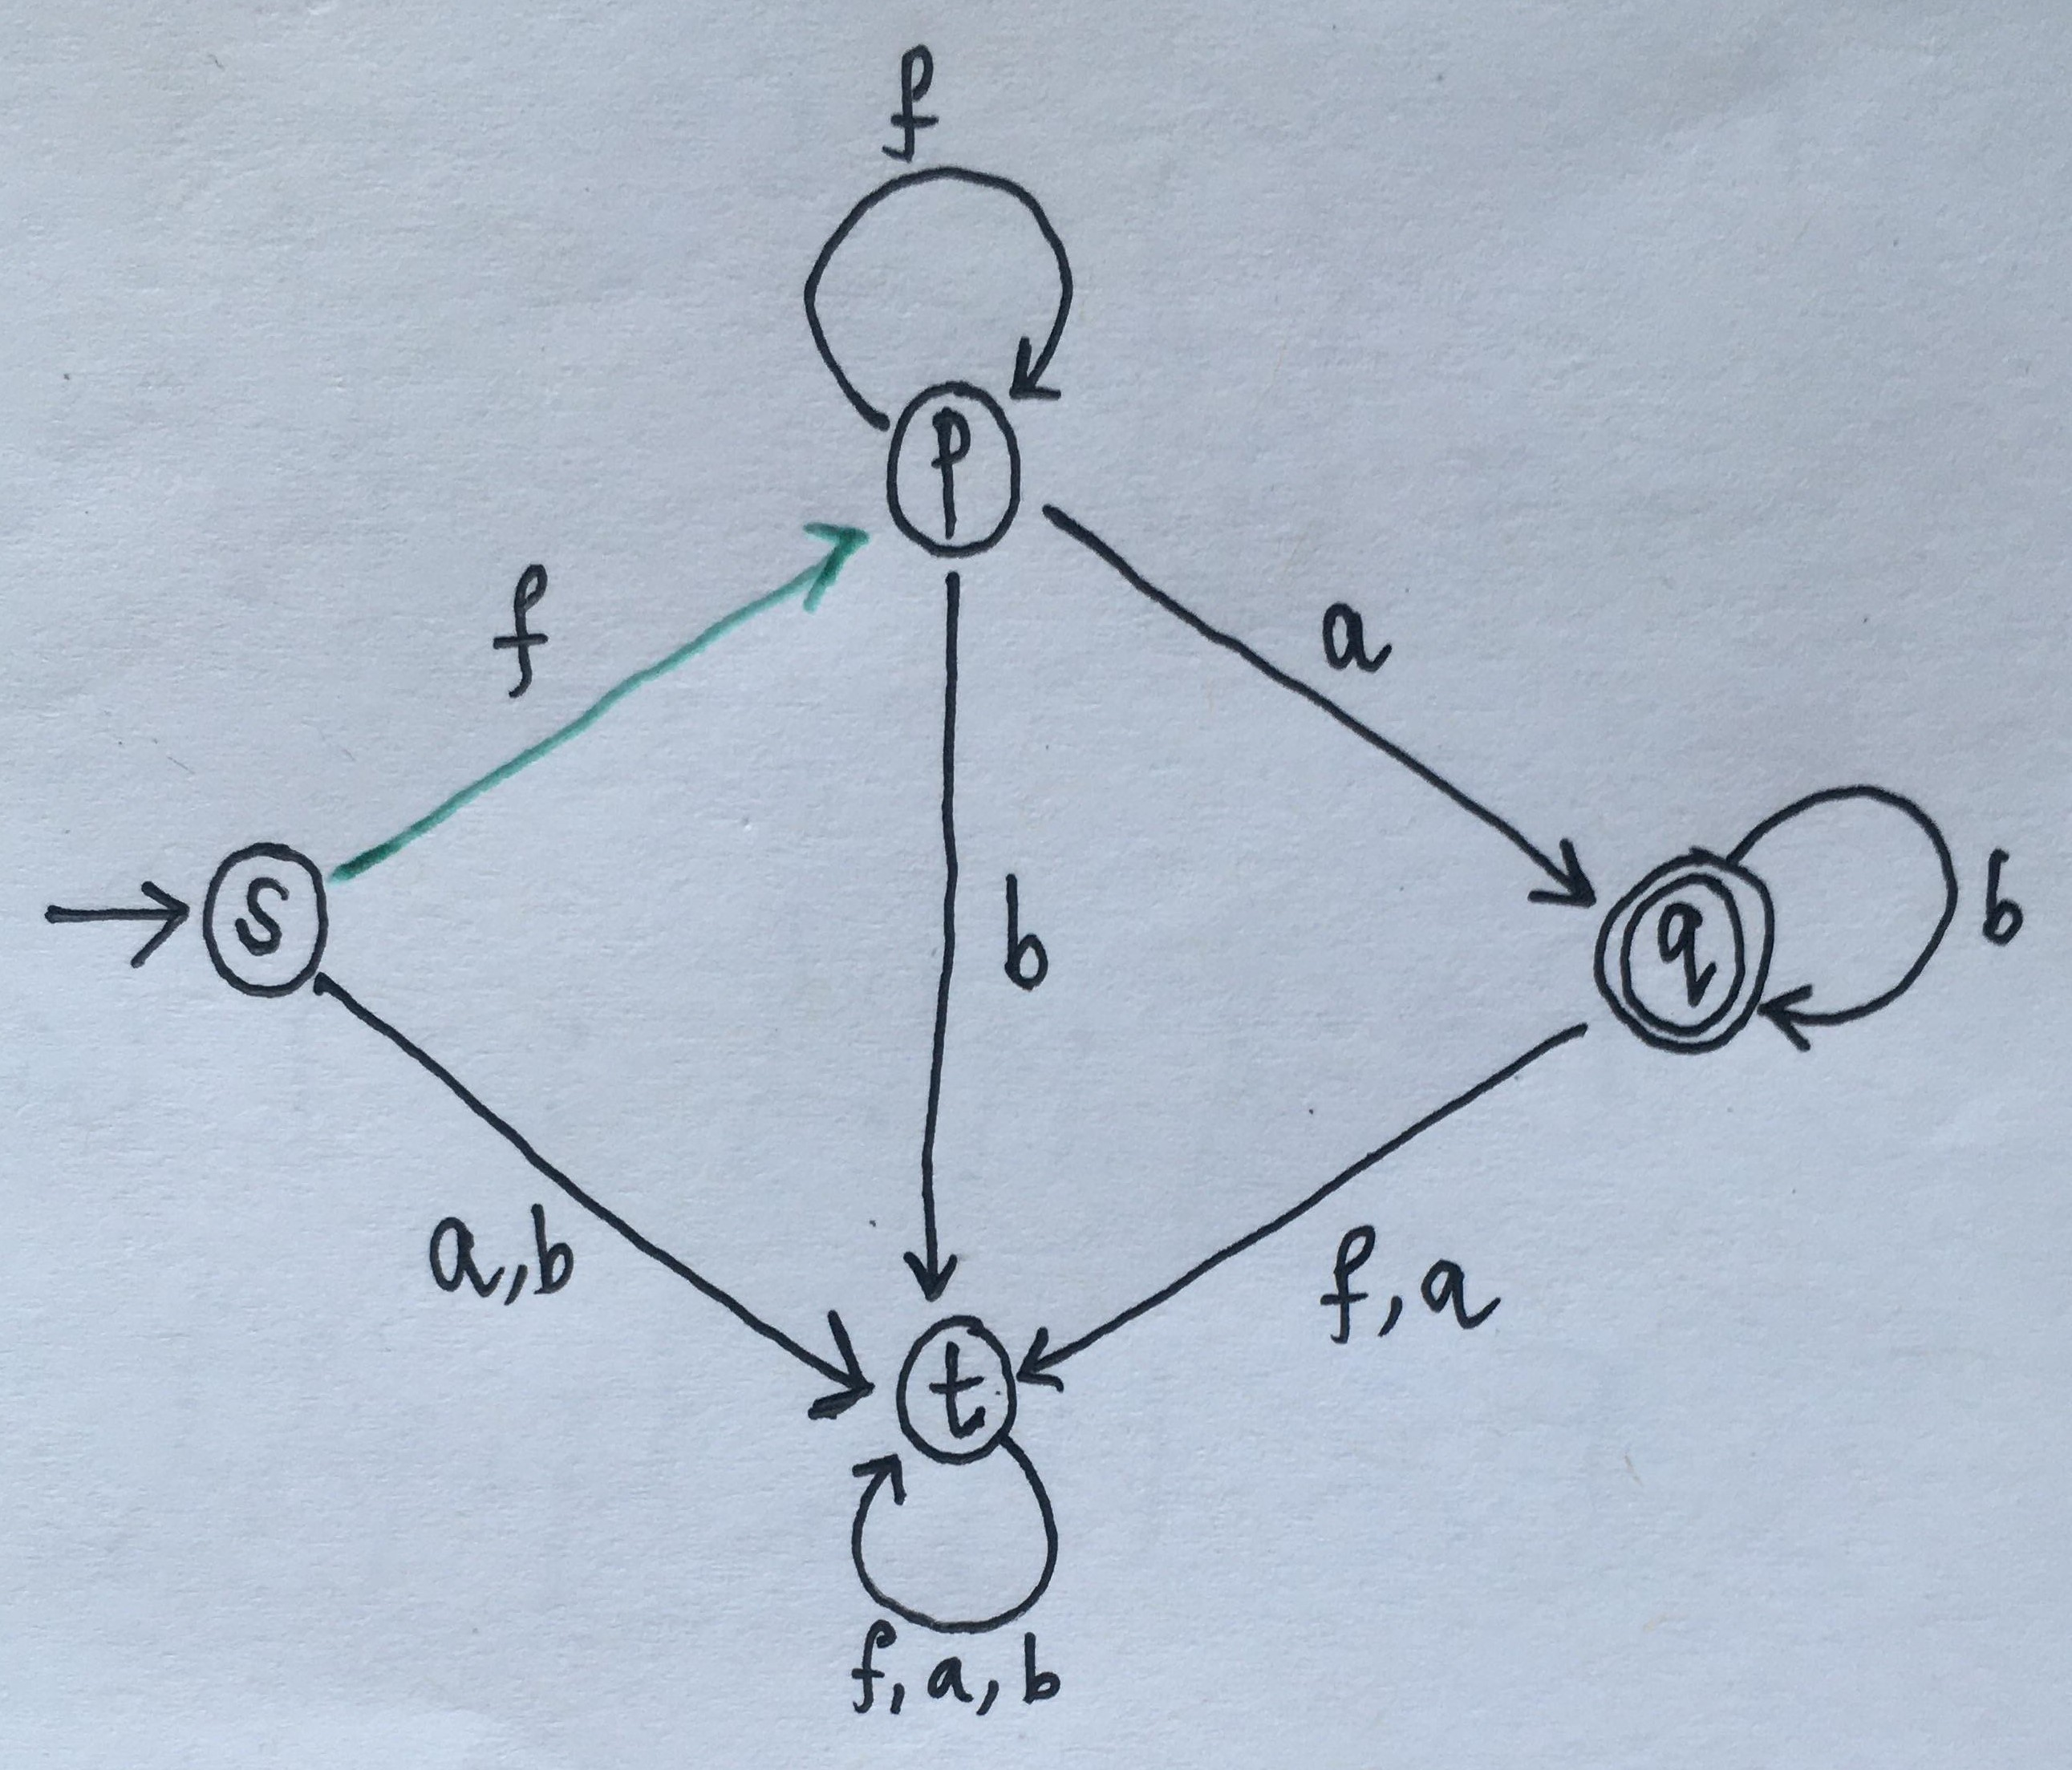
\includegraphics[width=250px]{figure1.1.jpg}
\caption{A Transition Diagram of M}
\label{image-Figure1}
\end{figure}

\end{exmp}

My example shows the DFA
$M=(\{s,p,q,t\},\Sigma,\delta,s,\{q\})$ over $\Sigma=\{a,b,f\}$. In a transition diagram, the arrows are called arcs, the final states are shown by a double circle around them and the start state is shown by $\rightarrow$ going into it. It is the only arc which does not have a start and end point.  

I designed M with a Language $L(M) = \{f^mab^n \in \Sigma^* \mid n,m \in \mathbb{N} \text{ and } m \geq 1\}$.
At each state, on reading a letter in $ \Sigma$
there is a singular arc for each letter of the alphabet, meaning given any string $x\in\Sigma^*$ the automata will end in one final state. If this final state is $q\in F$ then the string is accepted, i.e.  $x\in L(M)$.  It is clear that automata reject or accept strings based upon what their final state is, i.e. the language of an automaton is dependent on (amongst other things) the set of accepting states $F$. An example of an accepted string is $x=fab$, whereas $y=fabab \notin L(M) $.

\subsection{The Transition Function $\delta$}
\label{delta}
The transition function, $\delta$, from \ref{DFAdef} can be thought of as a function which performs the transformation of arcs. So, 
$\delta(s,f)=p$ means if the DFA is in state $s$ and reads symbol $f$, then transition to state $p$, highlighted by green arc in figure 1.1.

The \textbf{Extended Transition Function}
$\hat{\delta}: Q\times \Sigma^* \rightarrow Q$ describes a sequence of arcs. For example, $\hat{\delta}(s,x)=q$  means at state $s$ on reading string (input) $x$ the automaton will transition through states, at each state it reads the next symbol of $x$ and transition to the next state to do the same until it has read all of $x$ and hence will be in state $q$. The Formal definition of $\hat{\delta}$ is given by recursion on the length of a string:
\begin{itemize}
    \item[]$ \hat{\delta}(p,\varepsilon)=p$
    \item[]$ \hat{\delta}(p,xa)=\delta(\hat{\delta}(p,x),a)$ \thinspace \ where $x\in\Sigma^*, a\in\Sigma$ and $p\in Q$. 
\end{itemize}

This motivates a formal definition for the \textbf{Language of a DFA} M, $$L(M)=\{x\in\Sigma^*\mid\hat{\delta}(s,x)\in F\}$$ [3]. Which is the set of all strings whose sequence of symbols brings the DFA from it's start state to an end state in $F$. This corresponds to strings whose runs end in $F$.  

\section{Nondeterministic Finite Automata (NFA)}
\label{NFA}  
In this section, I will define nondeterministic finite automata (NFA) with and without $\varepsilon$-transitions, their respective transition functions (which are embedded into their definitions) alongside many examples. 

The basic premise for NFA is at a node on a given input symbol it has a choice of where to transition to, i.e. there can be multiple transition arcs from a node all with the same input. This means there can be multiple runs of the NFA for a string (runs are the states the automaton transitions to and paths are the symbols producing these runs).  In an NFA there are different runs which have the same path whereas in a DFA each path has a unique run. If a string produces a run that ends in an accepting state then the NFA accepts said string. 

\begin{definition}[NFA]
\label{NFAdef}
A Nondeterministic Finite Automaton, named N, is a 5-tuple $N=(Q,\Sigma,\Delta,S,F)$ where, 
\begin{itemize}
    \item[] $Q=$ A finite set of states
    \item[] $\Sigma=$ Some finite alphabet
    \item[]  $\Delta: Q\times \Sigma \rightarrow P(Q) $ where $\Delta$ is the transition function for N see section \ref{Delta}
    \item[] $S\subseteq Q$ The set of start states
    \item[] $F\subseteq Q$ The set of final accepting states
\end{itemize}
\end{definition}

\subsection{The Transition Function $\Delta$}
\label{Delta}
The co-domain of  $\Delta$  is the power set of $Q$, $P(Q)$, which is the set of all possible subsets of $Q$. This means for $q\in Q$, $a\in \Sigma$ we have 
$\Delta(q,a)$ $\subseteq Q$ i.e as already stated the transition function gives possibly zero or more states that the automaton can end up in after reading $a$. For reiteration, this is the key difference between a NFA and a DFA. A NFA has a `choice' of where to go on reading a string,  the `choice' the automaton will make is not determined by the machine hence the name non-deterministic. Rather the automaton runs all choices simultaneously and if any of these choices end up in an accepting state, the string is accepted.  [4, section 2.5, p.48-49]

\begin{definition}
\label{DeltaDef}
The \textbf{Extended Transition Function} takes a set of states $A$ and a string $x\in\Sigma^*$ as inputs and produces a set of states $B$ where $B$ is all the states the NFA could end in on input $x$ from a state in $A$, denoted $\hat{\Delta}(A,x)=B$. 
Similarly to \ref{delta} we define the Extended Transition Function, $\hat{\Delta}: P(Q)\times \Sigma^* \rightarrow P(Q) $, by induction on the length of the string.


Base case: let $A\in P(Q)$,  then $\hat{\Delta}(A, \varepsilon)= A$. 

Inductive hypothesis: for all strings $x$ with $|x|\leq k \in \mathbb{N}$ let $\hat{\Delta}(A, x)= B \subseteq Q$ be defined. 

Inductive step: suppose we have a string $y=xa$ where $a\in \Sigma$, that is $|y|=k+1$. By the inductive hypothesis we know $\hat{\Delta}(A,x)=B$ for $B$ $\subseteq Q$, hence we define

$\hat{\Delta}(A,y)=\hat{\Delta}(A,xa)=\bigcup\limits_{q\in B} \Delta(q,a) = \bigcup\limits_{q\in \hat{\Delta}(A,x)} \Delta(q,a)$.

Informally the definition means starting from a state in $A$, and on reading string $y$, we first read string $x$. Then $\hat{\Delta}(A,x)$ gives all the states you can be in after reading string $x$, namely $B$. From each of these states read $a$ via the transition function, and the  union of all the states you transition to is all the states you could end in denoted $\hat{\Delta}(A,y)$. 
[1, section 2.3.3, p.58] [3]

\parskip 0.1in The \textbf{Language of NFA} N is given by $L(N)=\{x\in\Sigma^* \mid \hat{\Delta}(S,x)\cap F\neq \emptyset\}$. The intuition is $\hat{\Delta}$ gives all the states $N$ ends in after reading $x$ from a given set of states which is set here to be $S$. The language is all the strings which give $\hat{\Delta}$ to produce a set with at least one element of $F$, that is their intersection is nonempty. This is the collection of strings which contain a run that starts at a start state and on reading input $x$ end in an accepting state of $N$. Note strings contained in the language need at least one run on input $x$ to end in an accepting state but not necessarily any more. 
\end{definition}

\subsection{NFA with $\varepsilon$ transitions denoted $\varepsilon$-NFA}
 $\varepsilon$-NFA are NFA which we allow transitions on the empty string $\varepsilon$. This means these transitions require and occur with, no input. We define $\varepsilon$-NFA as in definition \ref{NFAdef} but with an amended transition function $\Delta: Q \times (\Sigma \cup\{\varepsilon\}) \rightarrow P(Q)$, which allows $\varepsilon$-transitions. 



\begin{exmp}
The $\varepsilon$-NFA E below demonstrates that $\varepsilon$-NFA can be used to identify words in texts. $E$ is over $\Sigma = \{A, B, C, ..., Z, a, b, c, ...,z, , . , , \}$ (space-bar, full-stop and comma are symbols included in $\Sigma$).  The word $E$ identifies, or rather the language of $E$ is, 
$L(E)=\{Cat, Cats, cat, cats\} $ (`Cat(s)' is included to account for if it is the first word of a sentence). 

One can see on reading the first symbol of an input string, $E$ either stays in the start state, 0, or moves to some state in $\{1,5,9,14\}$ via an $\varepsilon$-transition, where it then reads the first symbol.  If this symbol is $C$ or $c$, $E$ progresses towards one of the accepting states $F=\{4,8,13,18\}$ dependent on whether the successive symbols spell out the desired word.
[Ideas for this example came from 1, section 2.5, p.73]

\begin{figure}[ht]
\centering
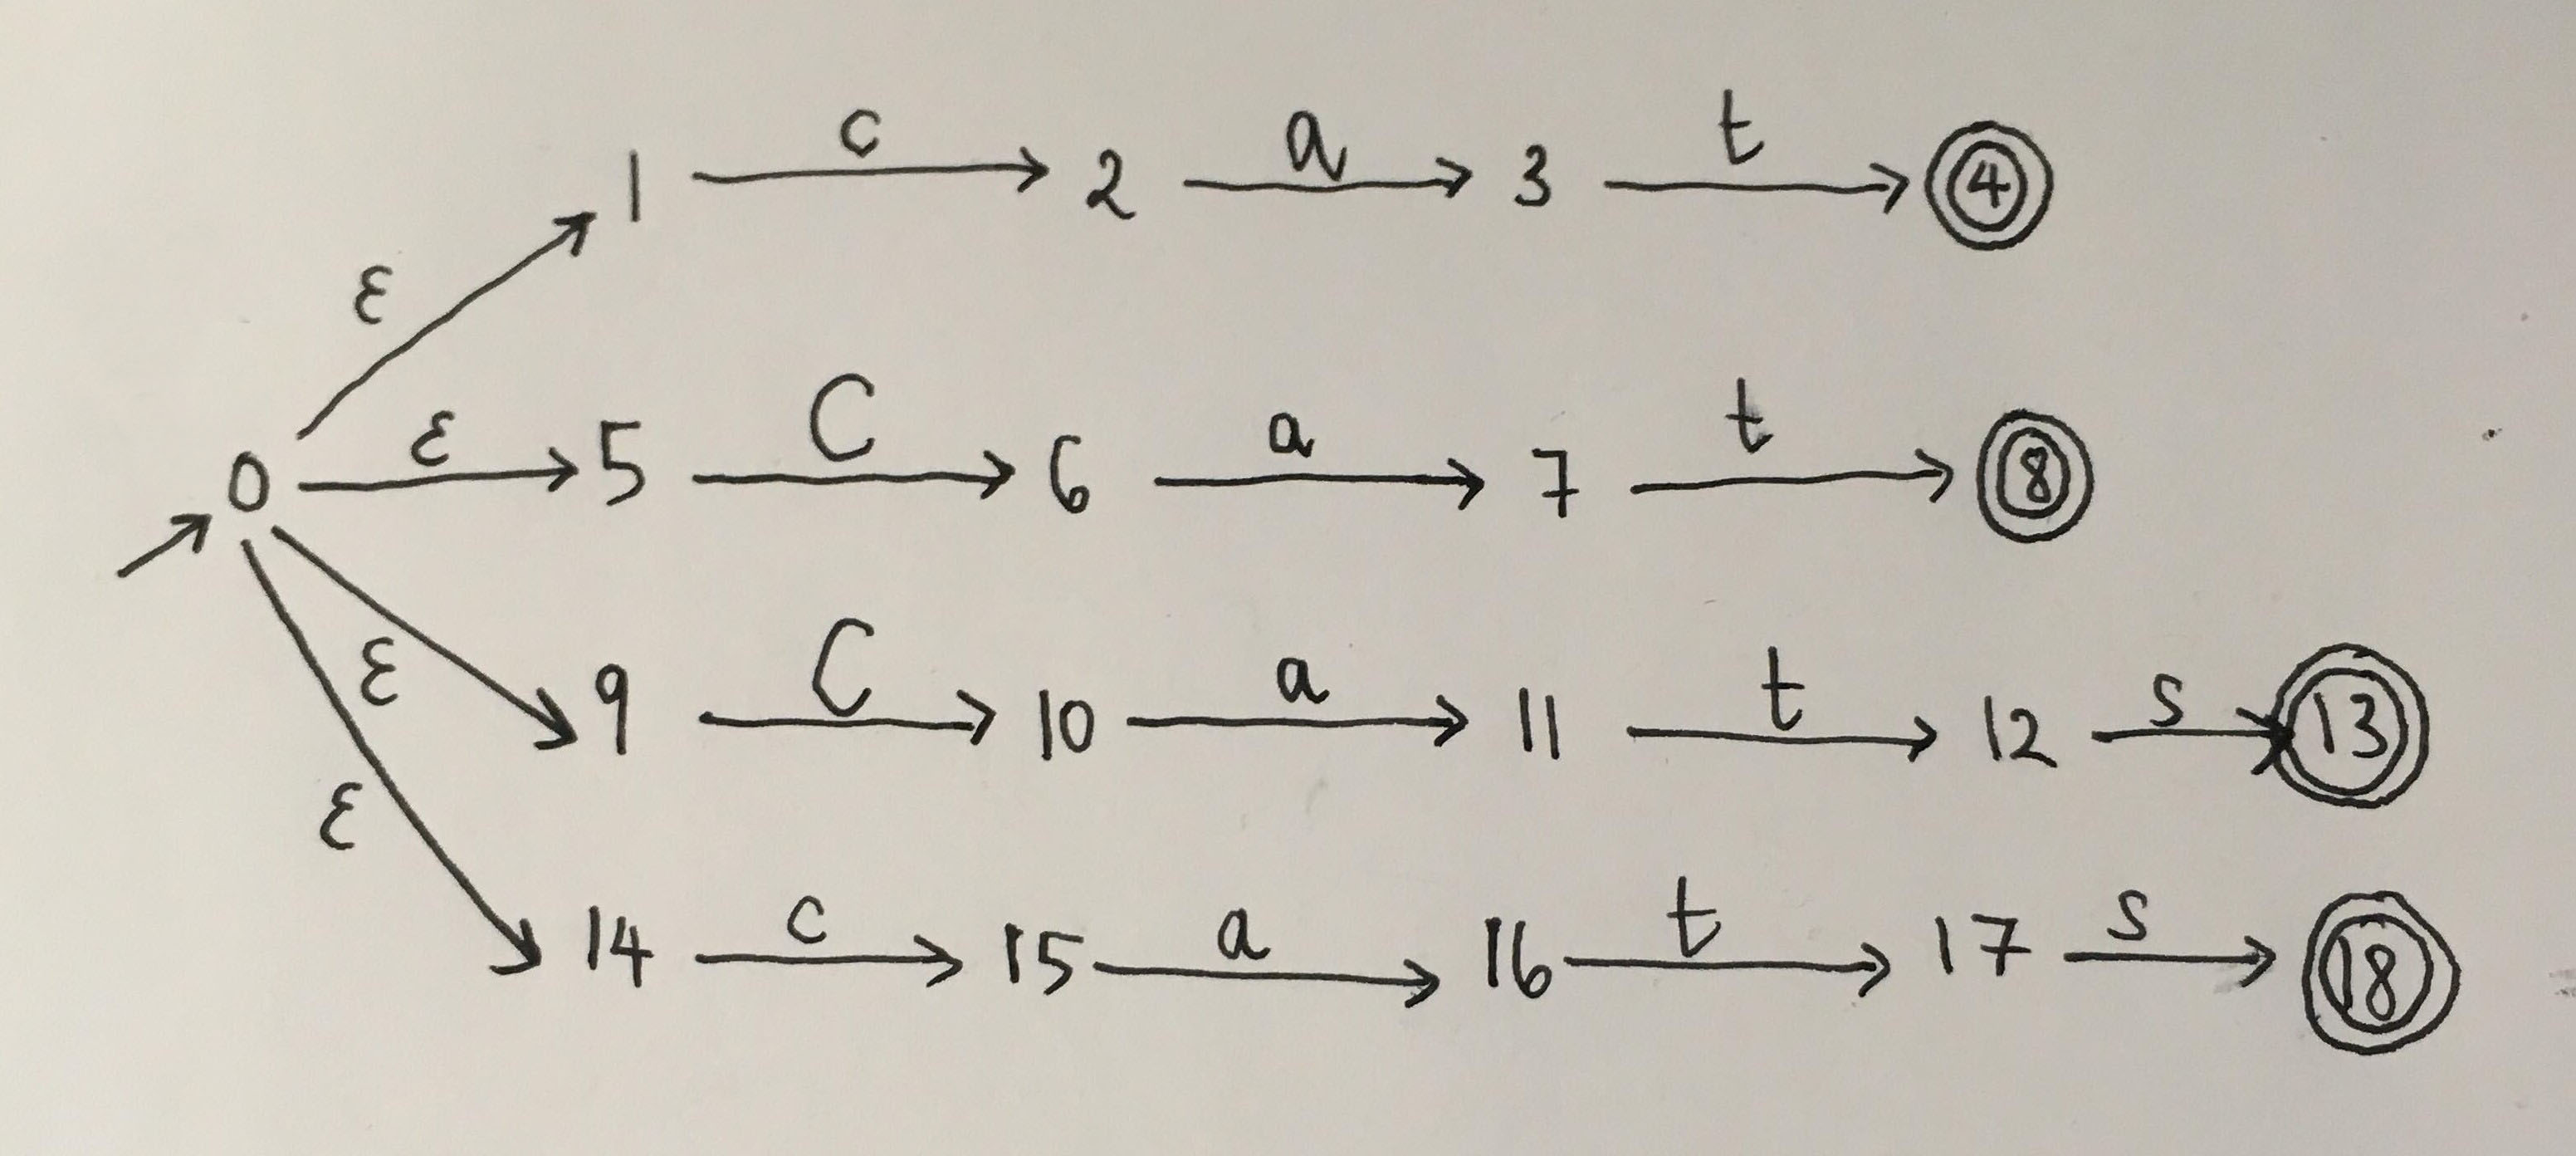
\includegraphics[width=300px]{figure1.2.jpg}
\caption{A Transition Diagram of E}
\label{image-Figure2}
\end{figure}
\end{exmp}

\begin{definition}($\varepsilon$-closure)
For any state $q\in Q$ the $\varepsilon$-closure of $q$ is

\noindent$\varepsilon$-\textit{cl(q)}$=\{p\ |\ p$ is reachable from $q$ via $\varepsilon$-transitions only\}. This definition is extended to $A \subseteq Q$ as $\varepsilon$-\textit{cl(A)}=$\bigcup\limits_{q \in A} \varepsilon$-\textit{cl($q$)}.
\end{definition}
\noindent [4, section 2.7 p.56]

\begin{exmp}
The $\varepsilon$-closure of every state $q$ is a set including $q$ (this could be the singleton set) since every state on no input is accessible from itself.
\end{exmp}

\begin{exmp}
In Figure \ref{image-Figure2} we have, $\varepsilon$-$cl(0)=\{$0, 1, 5, 9, 14\} and $\varepsilon$-$cl(q)=q$ for all $q\in Q\backslash \{0\} $.
\end{exmp}

\smallskip The \textbf{extended transition functions for $\varepsilon$-NFA $\hat{\Delta}$} is defined by induction on the length of a string $y=xa$, where $|y|=(k+1)$, $k\in \mathbb{N}$ and $a\in\Sigma$. Note $\{\varepsilon\}\notin\Sigma$ since $\varepsilon$ is not a character.  

Base case: $\hat\Delta(X,\varepsilon)=\varepsilon$-\textit{cl(X)} for $X\subseteq Q$

Inductive hypothesis: assume we have defined an extended transition function $\hat{\Delta}$ which provides the collection of states accessible from a set of states $X\subseteq Q$ on strings with length less than or equal to $k\in\mathbb{N}^+$. 

Inductive step: by construction $|x|\leq k $ so the set $A=\hat{\Delta}(X,x)$   exists by the  inductive hypothesis. Let $B=\bigcup\limits_{p\in A}\Delta(p,a)$, which is all the states accessible on reading $a$ from all the states in A. This is all the states we can access on input $y=xa$ without  $\varepsilon$-transitions as the final transition, as $A$ gives all the states we can reach on $x$ and then $B$ gives all the states we can transition to from $A$ on $a$. Finally we take the  $\varepsilon$-closure of $B$ to give   $\hat{\Delta}(X,y)=\hat{\Delta}(X,xa)=\varepsilon$-\textit{cl(B)}. This set is all the states an $\varepsilon$-NFA can access on input $y$ from some set of states $X$ and hence $\hat{\Delta}$ is defined correctly. [1, section 2.5.4, p.75]


\begin{note}
\label{DFA->eNFA}
For every DFA $M$ with $L=L(M)$ there is an equivalent $\varepsilon$-NFA $E$ such that $L=L(E)$.
This is easily shown by adapting $M$ to obey the $\varepsilon$-NFA definition. Let $M=(Q,\Sigma, \delta, s, F)$, then we define $E$ to be $E=(Q,\Sigma, \Delta, S, F)$ where $S=\{s\}$ and for $q\in Q$, 

$\Delta(q,\circ)= 
\begin{cases}
\{p\} \text{ if } \delta(q,a)=p \text{ and } \circ\in\Sigma\\
\emptyset \text{ if } \circ = \varepsilon 
\end{cases}.
$

Clearly, the language of $E$ and $M$ are the same as the transition function has been extended to take into account $\varepsilon$ input but it's output has been unchanged. Both have the same states, accepting states and effectively the same start state. [1, section 2.5, p.78] 
\end{note}
 

\chapter{Subset Construction}
\begin{theorem}
\label{thmSubConst}
Let $N=(Q_N,\Sigma, \Delta_N, S_N, F_N)$ be an NFA. Then there exists a DFA $M=(Q_M,\Sigma,\delta_M,s_M,F_M)$ that is equivalent to M, denoted $L(M)=L(N)$. 
\end{theorem}

\noindent[4, section 2.6, p.54]

\begin{proof}
Define $M=(Q_M,\Sigma,\delta_M,s_M,F_M)$ where: $Q_M = P(Q_N) $ is the set of all subsets of $Q_N$; $\Sigma$ remains unchanged; $\forall a\in\Sigma$ and $A\in Q_M$ we construct  

\noindent ($\dagger$) $\delta_M(A,a) = \hat{\Delta}_N(A,a) = \bigcup\limits_{q\in A}\Delta_N(q,a)$;

\noindent $s_M=S_N$ and  finally $F_M = \{ A\mid A \cap F_N \neq \emptyset\}$.

We've defined $\delta_M(A,a)=\hat{\Delta}_N(A,a)$ which is the set of states reachable on input $a$ from states in $A$ to be interpreted by  $\delta_M$ as a single state in $M$. $s_M$ is the single start state for $M$ which equals the set of start states for $N$. $F_M$ means for any state $q\in A \in Q_M$, if $q\in F_N$ then $A\in F_M$. We have now designed an automaton $M$ which fits the DFA  \ref{DFAdef} definition from a NFA $N$. It remains to show that the automata are equivalent, i.e $L(N)=L(M)$.

To show $L(M)=L(N)$ we must show $\hat{\delta}_M(s_M,x)=\hat{\Delta}_N(S_n,x)$ for every string $x$. This equivalence means for any input string $x$, the set of states $N$ ends in equals the single state, made up of this set, which $M$ ends in. Hence if $\hat{\Delta}_N$ produces a state in $F_N$ then $\hat{\delta}_M$ produces a state whose set contains this state and by definition of $F_M$ this will be an accepting state. Hence the equivalence means either both automata accept or both reject the string $x$. We prove this by induction on the length of a string $x$. Let $|x|= k \in\mathbb{N}$. 

Base case: $\hat{\delta}(s_M,\varepsilon)=s_M = S_N=\hat\Delta(S_N,\varepsilon)$ by definition of $M$.

Let us assume  $\hat{\delta}_M(s_M,x)=\hat{\Delta}_N(S_n,x)$ holds for all strings of length $k$. 
Let $y$ be the concatenation of $x$ and $a\in\Sigma$, that is $y=xa$, $|y|=k+1$. So,
% So $\hat{\delta}_M(s_M,x)=B \iff \hat{\Delta}_N(S_n,x) =B$ for some set $B\in Q_M$
\begin{align*}
   \hat{\delta}_M(s_M,y)&= \hat{\delta}_M(s_M,xa)\\
   &=\delta_M(\hat{\delta}_M(s_M,x),a) \ \text{by definition of $\hat{\delta}$} \\
   &=\bigcup\limits_{q\in\hat{\delta}_M(s_M,x)}\Delta_N(q,a) \ \text{ by ($\dagger$) in construction of M with }A=\hat{\delta}(s_M,x) \\
   &=\bigcup\limits_{q\in\hat{\Delta}_N(S_N,x)}\Delta_N(q,a) \ \text{by inductive hypothesis}\\
   &=\hat{\Delta}_N(S_N,xa) \ \text{by $\hat{\Delta}$ def \ref{DeltaDef}}\\
   &=\hat{\Delta}_N(S_N,y)
\end{align*}
\end{proof}

First I will discuss the relationship between NFA and DFA, then, at the end of the chapter I will relate how $\varepsilon$-NFA tie into this relationship. 

\begin{note}
By note \ref{DFA->eNFA} all DFA are NFA (since the $\varepsilon$-NFA can be considered as a NFA by defining $\Delta$ without the $\varepsilon$ case). Hence, for every DFA M there is an NFA N such that $L(M)=L(N)$, i.e. every language of a DFA is also the language of a NFA. 

Moreover,  by Theorem \ref{thmSubConst} for every NFA N there exists and DFA M such that $L(M)=L(N)$, i.e. every language of a NFA is also the language of a DFA. Whence the language of DFA equals the language of NFA and the two finite automata have equivalence.  This is equivalent to,
\end{note}  

\begin{theorem} 
\label{DFA=NFA}
The language $L$ is accepted by some DFA iff $L$ is accepted by some NFA.
[1, section 2.3, Theorem 2.21 p.64]
\end{theorem}

This proves that NFA are no more powerful than DFA as the language they accept is the same. This, potentially surprising result, is utilised since NFA are generally easier to design and can be used to program more advanced software for harder problems which can then be transformed or `complied' using subset construction into a DFA in order to be run on a computer. [1][4] 



\begin{exmp}
I have converted the NFA N, given in the transition table on the left, to a DFA M, given in the transitions table on the right, using subset construction. Below is a transition diagram of each to make it clearer that they accept the same language. 

The language they accept is $L(N)=L(M)=\{x00 \text{ or } y1 \mid x,y \in\Sigma^*\} =\{$the string must end in at least two zeros or a 1\} 

\noindent[This is exercise 2.3.3 given in 1 for the reader to complete and determine the language for, section 2.3.7, p.66]
\begin{flalign*}
    &\begin{array}{ r || c | c }
    N & 0 & 1 \\
    \hline
    \rightarrow p & \{p,q\} & \{p\} \\
    \relax      q & \{r,s\} & \{t\} \\
                r & \{p,r\} & \{t\}\\
                *s & \emptyset & \emptyset\\
                *t & \emptyset & \emptyset
    \end{array}&
    &\begin{array}{ r || c | c }
    M & 0 & 1 \\
    \hline
    \rightarrow A=\{p\} & B=\{p,q\} & A=\{p\} \\
    \relax      B=\{p,q\} & D=\{p,q,r,s\} & C=\{p,t\} \\
                *C=\{p,t\} & B=\{p,q\} & A=\{p\} \\
                *D=\{p,q,r,s\} & D=\{p,q,r,s\} & C=\{p,t\} 
    \end{array}&
\end{flalign*}

\begin{figure}[ht]
\centering
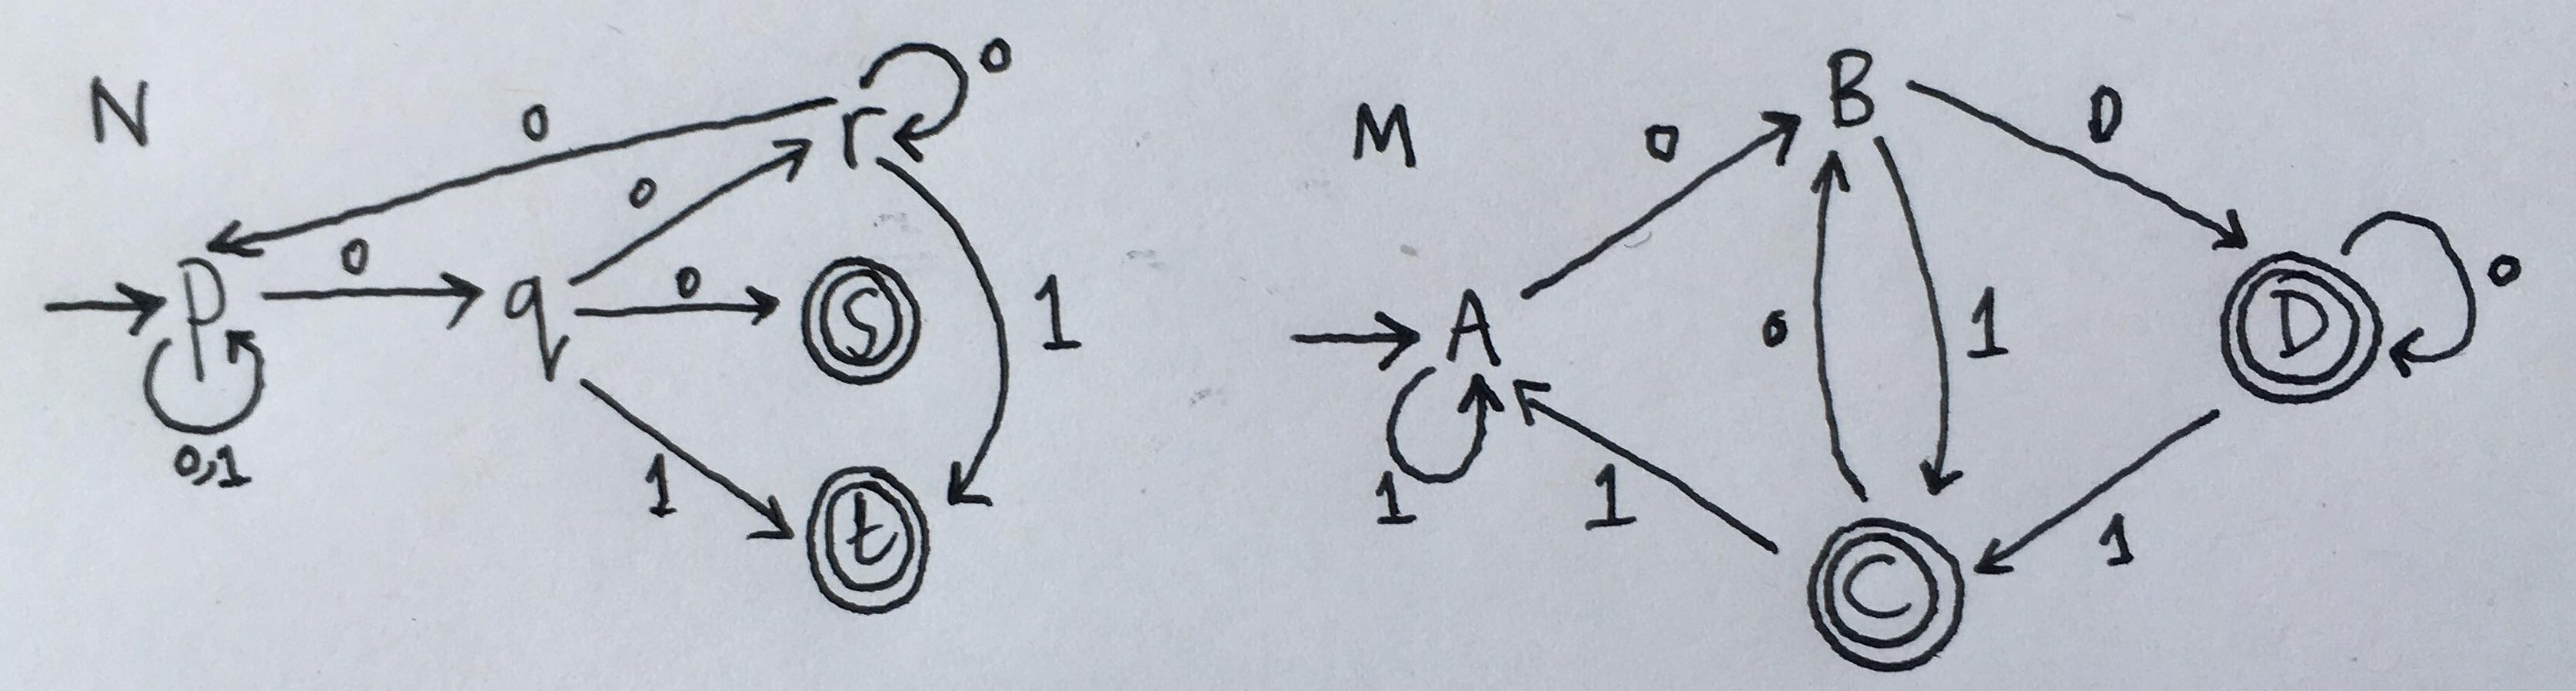
\includegraphics[width=400px]{figure1.3.jpg}
\caption{Transition Diagram of N (left) and M (right)}
\label{image-Figure3}
\end{figure}

\end{exmp}

\begin{note}
For a NFA with $n$ states, the DFA obtained from Theorem \ref{thmSubConst} has by definition $2^n$ states.  However, it is likely that many of these states are unattainable from the start state, i.e. there is not a path of acrs from the start state to said state, rendering it useless. This is why we form a transition table for the construction of the DFA which only allows for states reachable from the start state. However, it is important to note that a subset constructed DFA \textit{can} be accessible to all $2^n$ states, which is an exponential growth of states. This is a potential limitation for the running time/ processing power of machines which utilise this method of subset construction to form DFA from NFA. [1, section 2.3.6, p.64]
\end{note}

\begin{theorem}
\label{DFA<->eNFA}
A language $L$ is accepted by some $\varepsilon$-NFA iff $L$ is accepted by some DFA. [1, section 2.5 theorem 2.22, p.78]
\end{theorem}

\begin{proof}
By note \ref{DFA->eNFA} every language $L$ of a DFA is also the language of an $\varepsilon$-NFA.

For the only if direction, assume $L$ is the language of some $\varepsilon$-NFA $E=(Q_E,\Sigma,\Delta, S, F_E)$. We will construct an equivalent DFA $M$ by eliminating $\varepsilon$-transitions and subset construction in order to achieve $L(M)=L$.

Let $M=(Q_M,\Sigma, \delta, s, F_M)$ which is defined as follows, $Q_M=P(Q_E)$. The start state of $M$ is the set of all accessible states via $\varepsilon$-transition from the start states of $E$, that is $s=\varepsilon$-$cl(S)$. The final states of $M$ is $F_M=\{X \mid X\in Q_M \text{ and } X\cap F_E \neq\emptyset \} $.  For defining the transition function of $M$ let $X\in Q_M=P(Q_E)$ and let $\delta(X,a)=\Delta(X,a) $, that is all the states accessible in $E$ on input $a$ from all the states in $X$.

Now we must show that $L(E)=L(M)$ or equivalently $\hat{\Delta}(S, y)=\hat{\delta}(s,y)$ for $y=wa\in\Sigma^*$. This proof is very similar to that in \ref{thmSubConst} but $\hat{\Delta}$, the extended transition function for $\varepsilon$-NFA, takes into account the epsilon closure of states.

Base case: \begin{align*}
\hat{\delta}(s,\varepsilon)&=s\\
&=\varepsilon\text{-}cl(S)\\
&=\hat{\Delta}(S,\varepsilon) \text{ by extended transition function definition } 
\end{align*}
Inductive hypothesis: assume $\hat{\Delta}(S, w)=\hat{\delta}(s,w)$ holds.

Inductive step: 
\begin{align*}
\hat{\delta}(s,y) &=\delta(\hat{\delta}(s,w),a) \text{ by definition since } y=wa\\
&=\delta(\hat{\Delta}(S,w),a) \text{ by inductive hypothesis } \\
&=\Delta(\hat{\Delta}(S,w),a) \text{ by construction of }M\\ 
&=\hat{\Delta}(S,wa)\\
&=\hat{\Delta}(S,y)
\end{align*}
\end{proof}
[1, section 2,5 p.77-79]

\begin{note}
\label{FiniteEquivalence}
Combining theorem \ref{DFA<->eNFA} and theorem \ref{thmSubConst} we have that all finite automata are equivalent. So for any language $L$, there is an $\varepsilon$-NFA which accepts $L$ if and only if there is a NFA which accepts $L$ if and only if there is a DFA which accepts $L$.
\end{note}


\chapter{Regular Expressions}
Regular expressions give us an equivalent algebraic way to describe the language  of finite automata (this will be proved in this chapter). They frequently prove to be the preferred way to denote a language as often it can be complicated to extract the language from transition diagrams and the formal definition of finite automata. Regular expressions are pivotal in the construction of programs which scan and extract specific strings from text. 

A note for this chapter is since $\varepsilon$ and $\emptyset$ are formally different objects $\{\varepsilon\}\neq\emptyset$, the latter has no strings and the former has one string, the empty string.

\parskip 0.1in \textbf{Operators} [1, section 3.1, p86-87] Let $L$ and $L_1$ be two language and $x,y$ two strings:
% and x and y be two strings:  
\begin{enumerate}
    \item Union denoted $L\cup L_1=\{x\mid \ x\in L \ \text{or} \  x\in L_1\} $
    \item Concatenation denoted $L \cdot L_1=\{xy\mid\ x\in L, y\in L_1\}$. The Language $L^0=\{\varepsilon\}$ is the identity for concatenation. We have $L^2=L\cdot L$ which extends to $L^i=L\cdot L^{i-1}$ for $i\in\mathbb{N}^+$.
    \item (Kleene) Closure denoted
    $L^*=\bigcup\limits_{i=0}^{\infty}L^i=\{\varepsilon\}\cup L\cup L^2 \cup L^3\cup ...$ 
    \begin{itemize}
        \item The Kleene Plus is the $L^+ = \bigcup\limits_{i=1}^{\infty}L^i= L\cup L^2 \cup L^3\cup ...$
        
        Note $L^+$ may contain the empty string if $\varepsilon\in L$, however if $\varepsilon\notin L$ then $L^+=L^*-\{\varepsilon\}$
        
        [5, section 5.1, p.158]
        \item Although each $L^i$ can be finite, $L^*$ is an infinite set except for two languages:\\
        The empty language $\emptyset$, $\emptyset^* = \emptyset^0\cup\emptyset^1\cup...=\emptyset^0=\{\varepsilon\}$
        [1, example 3.1, p.87]\\
        The language consisting of the empty string     $\{\varepsilon\}$, $\{\varepsilon\}^0 \cup\{\varepsilon\}^1\cup...=\{\varepsilon\}$
        \\
        These are the only languages whose closure is finite.
    \end{itemize}
\end{enumerate}


\begin{definition}[Regular Languages and Regular Expressions]
\label{RegLangDef}
The collection of \textbf{regular languages} over some alphabet $\Sigma$ and the \textbf{regular expressions} which represent them are defined recursively below:
\begin{itemize}
    \item [(a)]$\emptyset$ (The empty language) is a regular language denoted by the regular expression $\emptyset$.
    \item [(b)]$\{\varepsilon\}$ is a regular language denoted by the regular expression  $\varepsilon$.
    \item [(c)]For $a\in\Sigma$, $\{a\}$ is a regular language, denoted by the regular expression $a$.
    \item [(d)] If $r_1$ and $r_2$ are regular expressions, then  $r_1+r_2$, \ $r_1\cdot r_2$, \ $r_1^*$ are regular expressions with regular languages $L(r_1)\cup L(r_2)$, $L(r_1)\cdot L(r_2)$, $(L(r_1))^*$ respectively.
    \item[(e)] No other languages over $\Sigma$ are regular and no other sequences of symbols are regular expressions. 
\end{itemize}
[4, Definition 2.2.1, p.38 and p39]
\end{definition}  

\noindent We often omit the concatenation symbol $\cdot$ in regular expressions and languages for ease. To reiterate a regular expression $r$ has a regular language denoted $L(r)$. 
A regular expression denotes exactly one regular language, but a regular language can have multiple equivalent regular expressions denoting it.
Two regular expressions $r_1$ and $r_2$ (over some $\Sigma$) are equivalent if and only if their respective regular languages $L(r_1)$ and $L(r_2)$ are equal. Like above we have, $r^+=r\cdot r^*=rr^*$.
\begin{exmp}
In this example I have answered the exercise from [1, exercise 3.1.1 (a), p.92]

Let us create a regular expression for the language $L=\{$the set of strings not containing 101\} over $\Sigma=\{0,1\}$.
We must identify that if a zero occurs after a 1, then another zero must occur (or nothing). One such regular expression is $r_1=0^*(1+00^+)^*0^*$. Another is $r_2=0^*(1+00^+)^*(0+\varepsilon)^*$. Hence
$L=L(r_1)=L(r_2)$ and $r_1$ is equivalent to $r_2$.
\end{exmp}


\begin{exercise}
Question 4 from study exercises. Give regular expressions, $r_i$ shown below, for the following subsets of $\{a,b\}^*$, ($\Sigma=\{a,b\}$),
\begin{itemize}
    \item [(a)]$\{x : x$ contains an even number of $a$'s\} then $r_a = b^*(ab^*ab^*)^*$.
    \item [(b)]$\{x:x$ contains an odd number of $b$'s\} then $r_b=a^*(ba^*ba^*)^*(ba^*)$.
    
    I have taken the pattern for an even number of $b$'s and then concatenated this with an expression containing a single $b$ which is irrespective of $a$'s.

    \item [(c)] $\{ x: x$ contains an even number of $a$'s or an odd number of $b$'s\}, 
    
    $r_c=b^*(ab^*ab^*)^*+a^*(ba^*ba^*)^*(ba^*)$
    
    This is simply a combination of parts (a) and (b). Note the string $bbbb$ is allowed since there is zero (an even) occurrences of $a$.
    \item[(d)] $\{ x: x$ contains an even number of $a$'s and an odd number of $b$'s\},
    
   I have answered this part in two approaches. The first (longer) approach is by brute force. The regular expression needs the first sub-expression to give an even number of both $a$ and $b$. That is every time a single $a$ or $b$ occurs this must be concatenated with eventually another single $a$ or $b$. We either have $ab$ or $ba$ depending on which single letter occurs first. Since $aa$ and $bb$ maintain an even number of both they can occur freely at every option. So,
    $((ab+ba)(aa+bb)^*(ab+ba)+(aa+bb))^*$. 
    
    The second sub-expression which will be concatenated with the first must continue to add an even number of $a$'s (make every single $a$ eventually pair with a single $a$) but leave one $b$ unpaired.  That is, 
    $((ab+ba)(aa+bb)^*a + b)$. 
    
    Hence the regular expression is, 
    
    $r_d=((ab+ba)(aa+bb)^*(ab+ba)+(aa+bb))^*((ab+ba)(aa+bb)^*a + b)$.
    
    The second simpler approach is to create such a regular expression by utilising the complement language of a DFA. Below I have created a DFA $D=(Q,\Sigma, \delta, s, F)$ (figure 3.1) whose language is the complement of statement (d). Namely, it's language is an odd number of $a$'s (shown right of the vertical dashed central line) or an even number of $b$'s (shown left of the vertical dashed line). To achieve statement (d) we take the language of the complement of $D$ that is $D_c=(Q,\Sigma,\delta,s,Q/F)$. We may use figure 3.1 to represent $D_c$, remembering that in this case we take the double circled states as non accepting states and the single circled states as accepting states. The language of $D_c$ is given by the regular expression for the left side of the dashed line (in $D_c$) $ba^*(ba^*ba^*)^*$ and the regular expression for the right side of the dashed line (in $D_c$) $ab^*ab^*(ab^*a)^*$. Hence the regular expressions is $r_d=ba^*(ba^*ba^*)^*+  ab^*ab^*(ab^*a)^*$.
    
    \begin{figure}[ht]
    \centering
    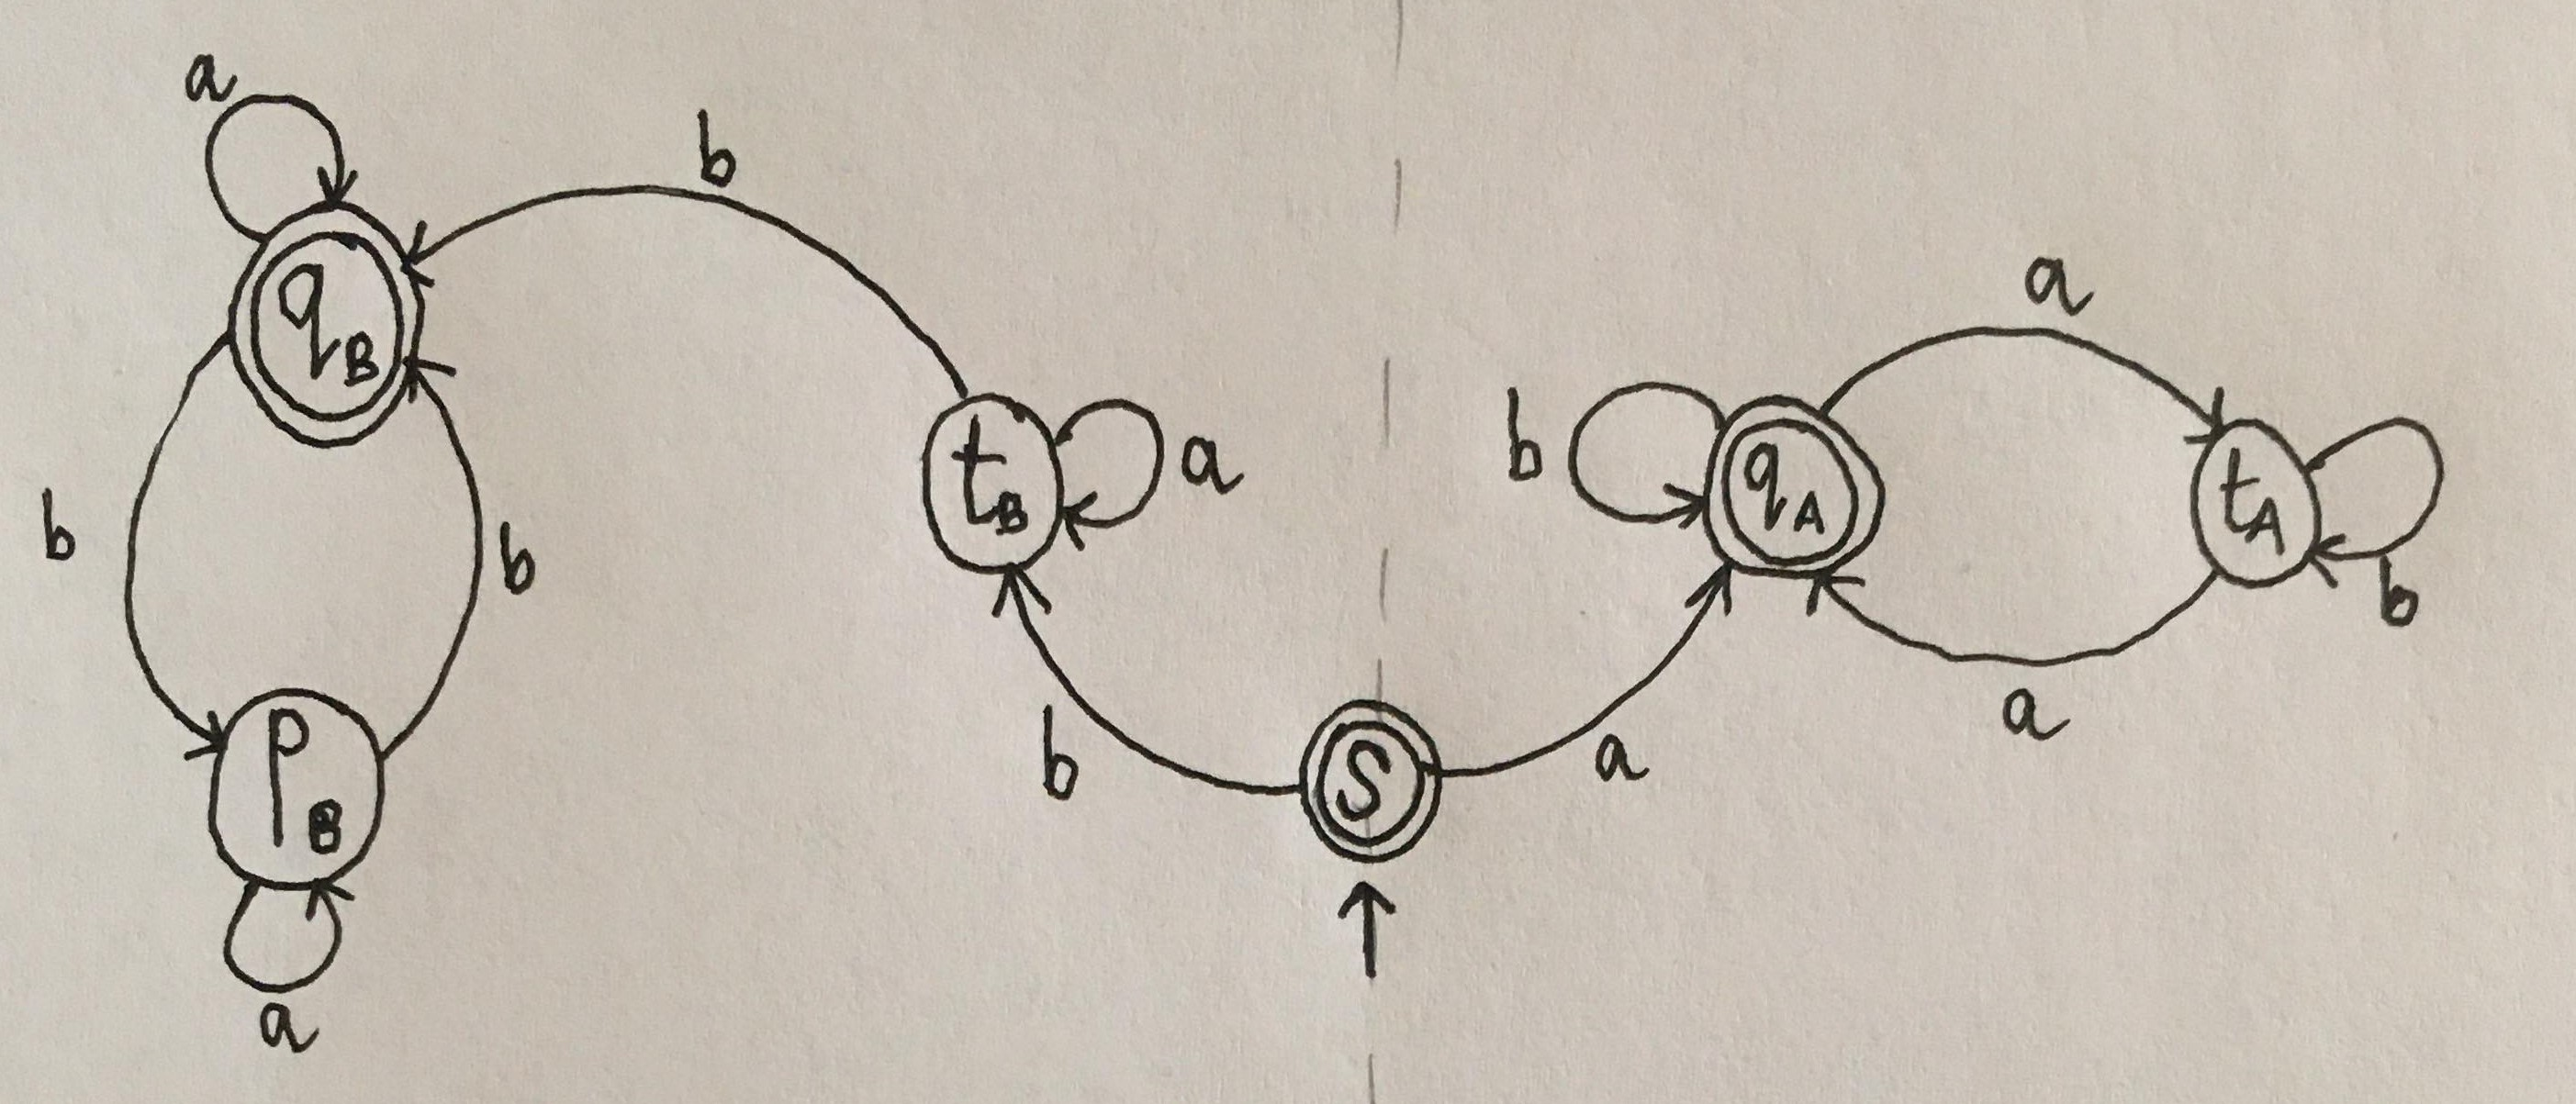
\includegraphics[width=400px]{figure1.9.jpg}
    \caption{Transition Diagram of D}
    \label{image-Figure1.9}
    \end{figure}
    \end{itemize}
\end{exercise}
    



\begin{theorem}(Kleene)
\label{Kleene}
A language is regular if and only if it is accepted by a finite automaton. [4, Section 2.8, Theorem 2.8.4, p.64]
\end{theorem}

This means a language $L$ is regular, i.e. there exists a regular expression $r_1$ with $L=L(r_1)$, if and only if there exists a finite automaton $B$ with $L=L(B)$. The language of the automaton equals the language of the regular expression which equals $L$ for any regular language $L$. Note by theorem \ref{DFA=NFA} automaton $B$ could be a DFA or a NFA or by theorem \ref{DFA<->eNFA} an $\varepsilon$-NFA.

By the end of this chapter we will have proven Kleene's theorem. In order to do this we prove Theorem \ref{RegEx->DFA} and Theorem \ref{DFA->RegExp} below. 

\begin{theorem}
\label{RegEx->DFA}
If we have a language $L=L(r)$ for $r$ a regular expression, then there exists a NFA $N$ such that $L=L(N)$.
\end{theorem}

\begin{proof}
By induction on the number of operators in $r$.

Base case: $r$ has no operators. This means by parts (a)-(c) of definition \ref{RegLangDef} $r$ is either $\emptyset$, $\{\varepsilon\}$ or $\{a\}\text{ for } a \in\Sigma$. We construct the equivalent NFA to r in each case, this is illustrated in figure 3.2 below by NFA $A$, $B$ and $C$.
\begin{figure}[ht]
\centering
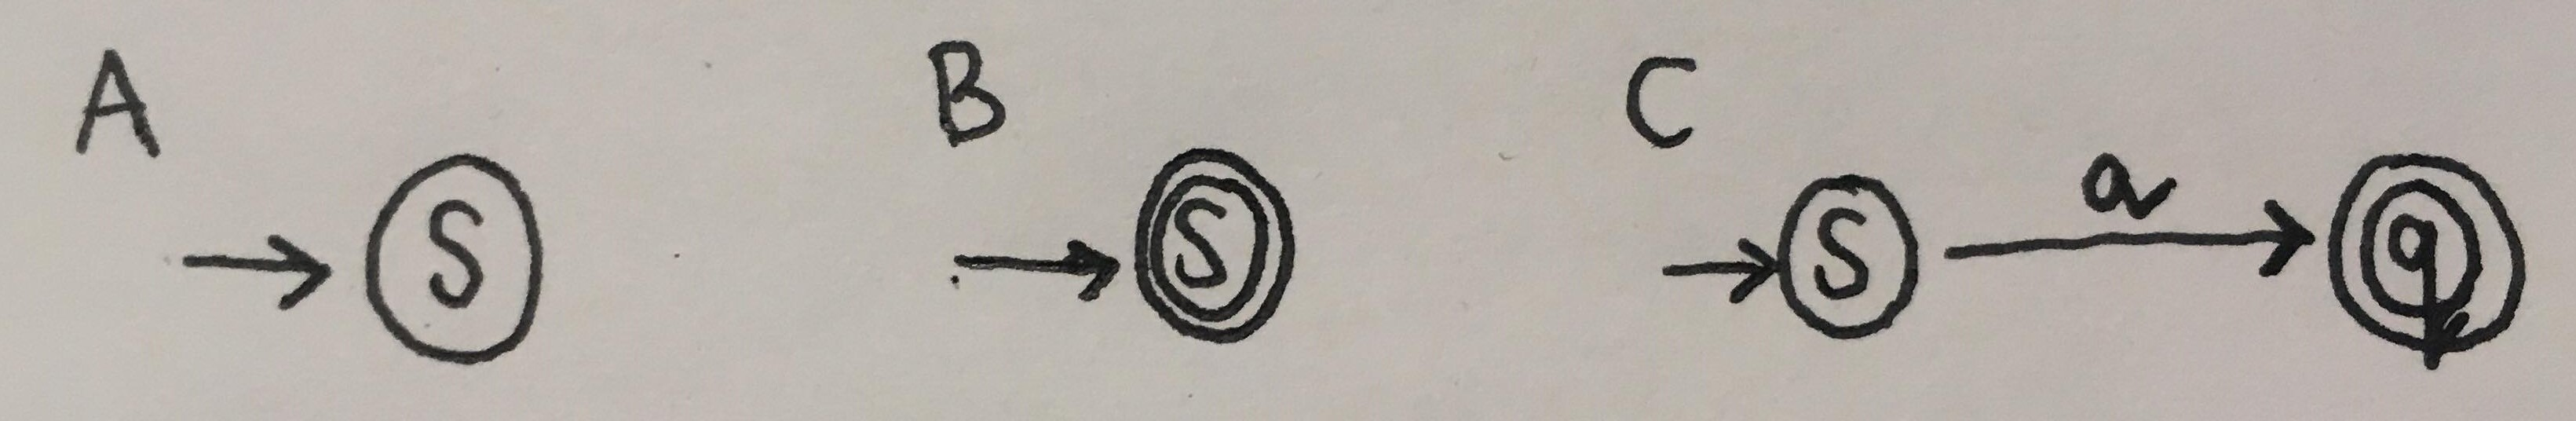
\includegraphics[width=400px]{figure1.4.jpg}
\caption{A Transition Diagram of A, B and C}
\label{image-Figure4}
\end{figure}

One can see the language of each automaton is equal to the regular expressions, that is $L(A)=\emptyset$, $L(B)=\{\varepsilon\}$ and $L(C)=\{a\}$.

Inductive step: we assume for all regular expressions $ r_i$ ($i\in\mathbb{N}$) with less operators than $r$ that there exists a finite automaton with an equivalent language. 
This means the outermost operators of r can be identified and the subsequent sub-expressions $r_1$ and $r_2$ have an equivalent NFA by the inductive hypothesis. Let these NFA be  $R_1=(Q_{R_1},\Sigma,\Delta_{R_1},S_{R_1},Q_{R_1})$ and $R_2=(Q_{R_2},\Sigma,\Delta_{R_2},S_{R_2},Q_{R_2})$ respectively, with $Q_{R_1} \cap Q_{R_2}=\emptyset$. That is $L_k = L(R_k)=L(r_k) \text{ for } k\in{1,2}$ (note in figures 3.3 and 3.4 the set $Q_{R_k}$ is denoted by the set $q_{R_k}$). Now we have reduced this proof to showing there exists an automaton for 3 cases, 
(i) $r= r_1 + r_2$,
(ii) $r = r_1 \cdot r_2$, and
(iii) $r=r_1 ^*$.

This is illustrated in the figures 3.3 and 3.4 below where the green circles represent automata defined in the inductive hypothesis. The start and end sets of each automaton are indicated by a single black circle.

\begin{figure}[ht]
\centering
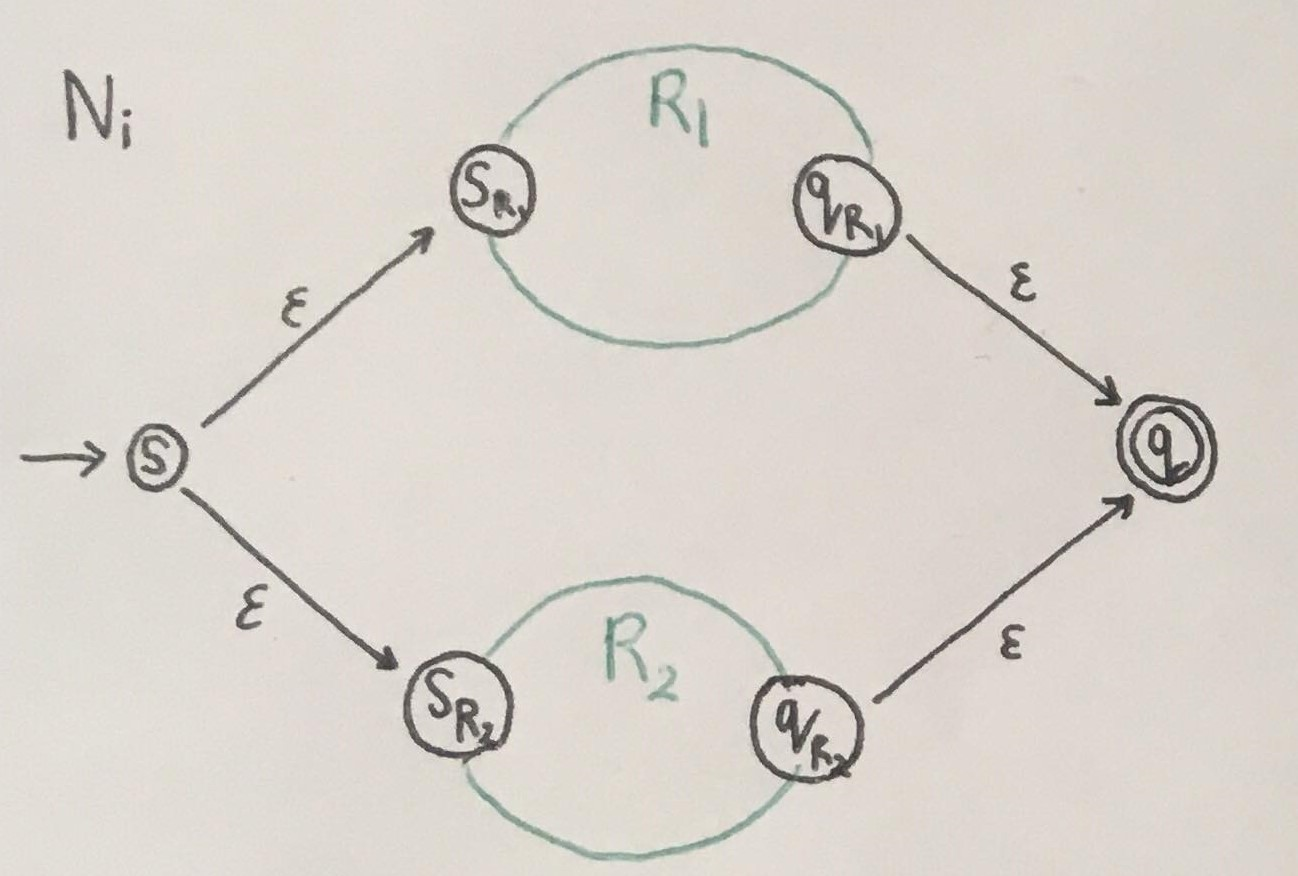
\includegraphics[width=250px]{figure1.5.jpg}
\caption{A Transition Diagram of $N_i$}
\label{image-Figure5}
\end{figure} 


For case (i), shown in figure 3.3, we have the $\varepsilon$-NFA $N_i=(Q,\Sigma, \Delta, \{s\} , \{q\})$ where $Q=Q_{R_1}\cup Q_{R_2}\cup s \cup q$, $\Sigma$ is the same language as $R_k$. The transition function is given by 

$\Delta(p,\circ)=
\begin{cases}
\Delta_{R_1}(p,\circ) \text{ if } p\in Q_{R_1} \text{ and } \circ=a\in\Sigma \\
\Delta_{R_2}(p,\circ)\text{ if } p\in Q_{R_2}\text{ and } \circ=a\in\Sigma \\
S_{R_1} \cup S_{R_2}\text{ if } p=s \text{ and }\circ = \varepsilon \\
q\text{ if } p\in q_{R_1} \text{ and }\circ = \varepsilon \\
q\text{ if } p\in q_{R_2} \text{ and }\circ = \varepsilon
\end{cases}$ 

This means on reading $x\in\Sigma^*$, $N_i$ has a choice to $\varepsilon$-transition to either a start state of $R_1$ or to a start state of $R_2$. If $N_i$ transitions to a start state of $R_1$ it will only be accepted if it is accepted in $L(R_1)$. This is because the only path to the final state of $N_i$ from here is to a final state of $R_1$. By the same reasoning if $N_i$ transitions to a start state of $R_2$ it will only be accepted if $x\in L(R_2)$. Hence the language of the automaton is, 

$L=L(N_i)=L(R_1)\cup L(R_2) = L(r_1) \cup  L(r_2)=L(r_1+r_2)=L(r)$.

For the remaining two cases, I only discuss the language of the NFA $N_{ii}$ and $N_{iii}$ as their construction can be extrapolated by the proof of case (i) and figure 3.4. 

\begin{figure}[ht]
\centering
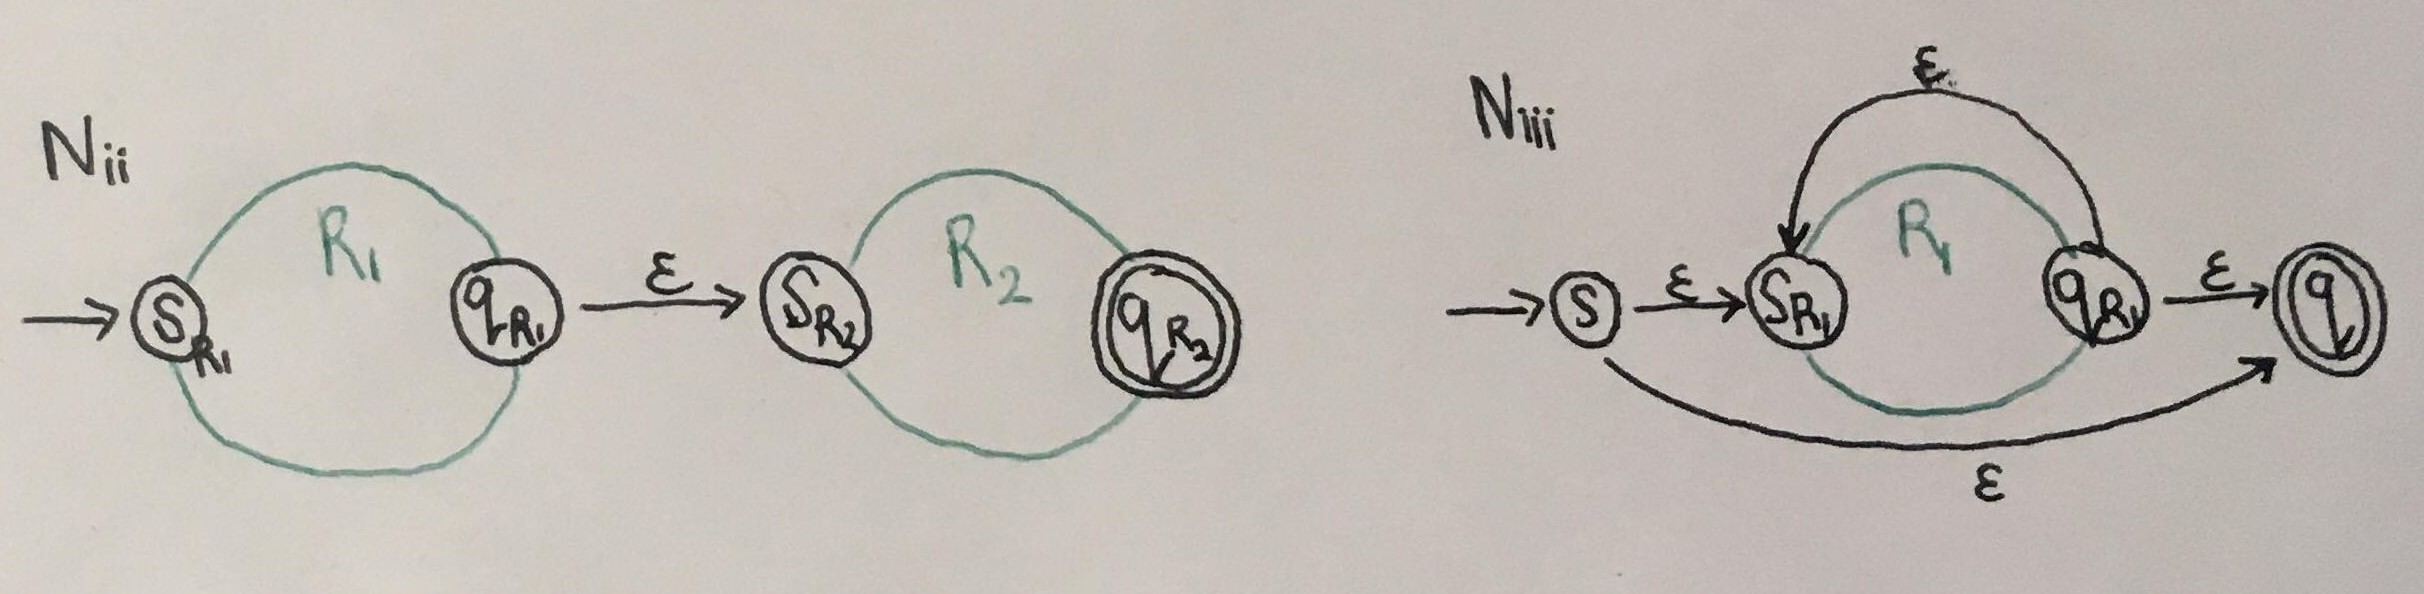
\includegraphics[width=450px]{figure1.6.jpg}
\caption{A Transition Diagram of $N_{ii} \text{ and of } N_{iii}$}
\label{image-Figure6}
\end{figure}

Case (ii):
Let $x\in\Sigma^*$ be accepted by $N_{ii}$. This means there is a partition $x=x_{R_1}x_{R_2}$ where $x_{R_1}$ must be an accepted string of $R_1$ and $x_{R_2}$ must be an accepted string of $R_2$.  This is because every path which is accepted by $N_{ii}$ must go through a start state of $R_1$ to a final state of $R_1$, given by $x_{R_1}$. Then in order to be accepted by $N_{ii}$ the automaton must choose to continue by an $\varepsilon$-transition to a start state of $R_2$ and then to a final state of $R_2$, given by $x_{R_2}$. $x$ is then accepted by $N_{ii}$ as it's final states are the final states of $R_2$, hence $x\in L(R_1)L(R_2)$. 

Conversely let $x\in L(R_1) L(R_2)$ that is $x=x_{R_1}x_{R_2}$. Since $x_{R_1}\in L(R_1)$, $x_{R_1}$ produces a state in $Q_{R_1}$. Then $N_{ii}$ can $\varepsilon$ transition from here to a start state of $R_2$ where since $x_{R_2}\in L(R_2)$ this produces a state in $Q_{R_2}$ which means $x$ is accepted by $N_{ii}$. Thereby the language of $N_{ii}$ is $L=L(N_{ii})=L(R_1)L(R_2)=L(r_1)L(r_2)=r_1\cdot r_2$.

Case (iii): 
Let $x\in\Sigma^*/\{\varepsilon\}$ be accepted by $N_{iii}$ (note $N_{iii}$ does accept $\varepsilon$). By construction of $N_{iii}$, $x$ must be formed of some accepting string of $R_1$ concatenated with any finite number of other accepting strings of $R_1$. This is because it is the only way to produce a path in $N_{iii}$ from it's only start state $s$ to it's only accepting state $q$. This exactly gives that $x\in L(R_1)^*$.

Let $x\in L(R_1)^*$, then either $x=\varepsilon$ which is accepted by $N_{iii}$ or we can partition $x$ by $x=r_1....r_n$ with $1\leq	n \in \mathbb{N}$ and $r_i\in L(R_1)$. In this case, after $N_{iii}$ has read each $r_i$ it simultaneously runs an $\varepsilon$-transition back to the start state of $R_1$ and another to the final state $q$. If the full strings has not been read then $N_{iii}$ can read $r_{i+1}$ from a start state of $R_1$, or if $r_{i+1}=r_n$ then since $N_{iii}$ also transitions to $q$ it accepts the string $x$. Whence the language of $N_{iii}$ is $L=L(N_{iii})=L(R_1)^*=L(r_1)^*=r_1^*$.

[1, section 3.2, p.103-105 ] [5, section 6.2, p.183-184]
\end{proof}

\begin{theorem}
\label{DFA->RegExp}
% If $L=L(A)$ for some DFA A, then there is a regular expression $R$ such that $L=L(R)$ [1, theorem 3.4, section 3.2, p.93]\\
If $L=L(M)$ for some DFA $M$, then $L=L(r)$ for some regular expression $r$. Where $L$ is the language over some $\Sigma$. [6, lecture 8, theorem 8.1, p.46]
\end{theorem}

\begin{proof}
Let $M$ be a DFA defined by $M= (Q, \Sigma, \delta, s, F)$ with $u,v \in Q$ and $X = \{q, q_1, ... , q_n\} \subseteq Q$.

We define $r_{u,v}^{X}$ to be the regular expression representing the set of all strings $x\in\Sigma^*$ such that $x$ is a path from $u$ to $v$ in $M$ (that is $\hat{\delta}(u,x)=v$) and this path $x$ only has runs within X, possibly excluding endpoints $u$ and $v$. As stated in an earlier chapter a run is the sequence of states that a path produces. 

We first show, by induction of the size of set $X$, there exists a regular expression representing the path between any two states in $M$ where said path has runs only within $X$ (excluding endpoints). We extend this by taking $X$ to be $Q$ and the two states to be $s$ and some end state $f\in F$. Then the regular expressions representing the language of $M$ is the summation of all these regular expressions for all states $f\in F$. 

Base case: $X= \emptyset $ . Let $A=\{a_1,...,a_m\}$ be the collections of symbols $a_i\in\Sigma$ such that $\delta(u,a_i)=v$.  This gives regular expressions, \\
for $u\neq v$ \\
$r_{u,v}^{\emptyset}=
\begin{cases}
a_1  + ... +  a_m\text{ for A non-empty},\\
\emptyset \text{ for A=}\emptyset
\end{cases}$\\
for $u=v$ \\
$r_{u,u}^{\emptyset}= r_{u,v}^{\emptyset} + \varepsilon$  
for clarification this is 
$r_{u,u}^{\emptyset}=
\begin{cases}
\varepsilon + a_1 + ... + a_m \text{ for A non-empty},\\
\emptyset + \varepsilon \text{ for A=}\emptyset
\end{cases}
$

Inductive hypothesis: 
we assume there exists a regular expression $r_{u,v}^{Z}$ as described above for all sets Z of smaller size than $X$. 

Inductive step: 
For any $uv$-path $x\in\Sigma^*$ which produces runs within $X$, $x$ either contains some state $q\in X$ or does not. 

If $x$ does not contain ${q}$ then since the set $X\backslash \{q\}$ is smaller than the set $X$, by the inductive hypothesis we have  $x$ is represented by the regular expression $r_{u,v}^{X\backslash\{q\}}$.

If $x$ contains $q$ then the path can be broken down into three sub-paths say $x=x_ax_bx_c$. The first sub-path $x_a$ is from $u$ to the first time the path arrives at $q$. The second sub-path $x_b$ is from the first time the path arrives at $q$ to the last time the path arrives at $q$ (note this section could be empty if $x$ contains $q$ once). The last sub-path $x_c$ is from the last time $x$ arrives at $q$ to $v$. 

As $x_a$ has $q$ as it's end point and $X$ can exclude the endpoints of a given path, $x_a$ run's can be described by the set $X\backslash \{q\}$ so by the inductive hypothesis $x_a$ is described by a regular expression $r_{u,q}^{X\backslash\{q\}} $. Since $x_b$ can contain multiple $q$'s we break down the subsection into sections from $q$ to $q$. Again since in every such section the run produced by $x_b$ can be formed from states in $X\backslash\{q\}$, which is a smaller set than $X$, the inductive hypothesis gives that the regular expressions $r_{q,q}^{X\backslash\{q\}}$ describes each section of $x_b$. Hence since each section concatenates together to give the path $x_b$, $x_b$ is represented by the regular expression $( r_{q,q}^{X\backslash\{q\}})^*$.  Finally by the same reasoning of $x_a$, the final sub-path $x_c$ is represented by $ r_{q,v}^{X\backslash\{q\}}$. Thus in this case $x$ is accepted by  $(r_{u,q}^{X\backslash\{q\}} )( r_{q,q}^{X\backslash\{q\}})^*(r_{q,v}^{X\backslash\{q\}})$.

Hence combining both cases for $x$ gives the definition of a regular expression denoting a path $x$ which gives runs within $X$ from $u$ to $v$. 

$r_{u,v}^{X} = r_{u,v}^{X\backslash\{q\}} + (r_{u,q}^{X\backslash\{q\}} )( r_{q,q}^{X\backslash\{q\}})^*(r_{q,v}^{X\backslash\{q\}}$) 

Thereby the language of $M$, $L=L(M)$, is described by the sum of all regular expressions from the start state, $s$, to all final states $f\in F$, i.e. the sum of all regular expressions of the form $r_{s,f}^{Q} $ for $f\in F$. That is $L=L(r)$ where $r=\Sigma_{f\in F} \ r_{s,f}^Q$.

Hence we have defined a regular expression for an arbitrary DFA M, meaning all DFA can be described by regular expressions. So by note \ref{FiniteEquivalence} this means all finite automata can be described by regular expressions. 
\end{proof}
[6, lecture 9, p.51-52]

\begin{exercise}
Question 2 from the study exercises.

For a string $x$ let $rev(x)$ denote the reverse of $x$. Let $\Sigma$ be a finite alphabet. Show that if $L\subseteq\Sigma^*$ is regular, then $rev(L) = \{x\in\Sigma^*\mid rev(x)\in L\}$ is also regular. 

Assume $L$ is regular. I will show that $rev(L)$ is regular by utilising the equivalence between finite automata and regular expressions. 
Let $D=(Q,\Sigma, \delta, s, F) $ be a DFA with $L(D)=L$, we know such an automaton exists since $L$ is regular. We adapt $D$ to create a new NFA $N$ with an amended transition function and a swapped start state for end states. That is $N=(Q,\Sigma, \Delta, F, \{s\})$,  for $a\in\Sigma$, $q\in Q$ we have $\Delta(q,a)=\{p \}\text{ if } \delta(p,a)=q$. 
We needed $N$ to be a NFA to allow for multiple start states which occur when we swap $s$ with the set of final states $F$. However since $\Delta$ takes the reverse direction of all transitions but adds no new transitions, the NFA is a just DFA with multiple start states i.e. there is exactly one choice for the automaton at all times. Clearly, the language of $N$ is the reverse of the language of $D$. Each transaction is reversed and the accepted and start states have been swapped, so if a string accepted by $D$, its reverse is accepted by $N$. Hence by theorem \ref{Kleene}  $rev(L)$ is regular since it is accepted by $N$. 
\end{exercise}

\chapter{Büchi Automata}
Büchi automata (BA) are extensions of the finite automata we have studied so far, they have a different input domain and hence a different acceptance condition. Büchi automata either accepts or rejects infinite inputs (strings) compared to DFA and NFA which process finite input only. A Büchi automaton is non deterministic which means on each (infinite) input there may be numerous possible paths which the automata can take. A Büchi automaton accepts an input if any of these paths visit a final state infinitely many times. There is a non equivalent deterministic Büchi automata but any reference to this automaton type will explicitly state the deterministic property.


\noindent[3][7, Büchi Automaton]

From the previous sections, $\Sigma^*$ denotes the set of all finite words over $\Sigma$. Now we introduce $\Sigma^\omega$ which denotes the set of infinite words over $\Sigma$, where $\omega=\{0,1,2,...\}=\mathbb{N}$. $\Sigma^\omega$ can be thought of as the concatenation of the alphabet with itself infinite times. For $\Sigma=\{a\}$ then $\Sigma^*=\{\varepsilon, a, aa, aaa, ...\}$ whilst $\Sigma^\omega=\{aaaa...\}$.

\noindent [10, Introduction, p.4][3]

An infinite word $\alpha \in \Sigma^\omega$ is an infinite sequence of symbols from $\Sigma$. Examples of infinite words $\alpha_0, \alpha_1, \alpha_2 \in\Sigma^\omega$ over $\Sigma=\{0,1\}$  are,
\begin{itemize*}
\item [] $\alpha_0 = 00000....$,
\item[]$\alpha_1=0011111111....$,
\item[]$\alpha_2=01101010001010....$ 
\end{itemize*}.
We can also represent an infinite word $\alpha$ as a function $\alpha:\omega \rightarrow \Sigma$ which means $\alpha$ takes an input over the natural numbers, say input $i$ and outputs the $i$-th symbol from $\Sigma$, i.e. $\alpha(i)$ denotes the symbol at the $i$-th position of $\alpha$. 


\noindent[9, Notation ,p.2][3]

\begin{definition}[BA]
\label{DefBA}
A Büchi Automaton, $B=(Q,\Sigma, \Delta, S, F)$ is a NFA  as in definition \ref{NFAdef} with an acceptance condition specified below.
[7, Formal definition]
\end{definition}

\begin{definition}
A \textbf{run}, $r$, of a Büchi automaton $B$ on input $\alpha=a_0a_1a_2... \in \Sigma^\omega$ is a sequence of states $q_0q_1q_2...$ which must follow:
\begin{itemize}
    \item $q_0\in S$ (the run should start at a start state)
    \item for all $i \in\{0,1,2,...\}, \ q_{i+1} \in \Delta(q_i,a_i) $ (every transition should be legal) 
\end{itemize}

\end{definition}
\noindent[3] [8, Büchi Automata, p.1]
\begin{definition}
The \textbf{infinite set} of a infinite word $\alpha\in\Sigma^\omega$ where $\alpha=a_0a_1a_2...$ is the set 
$In(\alpha)=\{ a\in\Sigma \mid \forall i \exists j \text{ such that } i\leq j \text{ and } a_j=a\}$. 

This means a symbol $a\in\Sigma$ is in the infinite set of $\alpha$ if it occurs in $\alpha$ infinitely many times. The set $In(\alpha)$ describes this by stating for all indices $i$ of the string $a$ there exists an index larger than $i$, namely $j$, such that the $j$-th index of $\alpha$ equals $a$.

The \textbf{infinite set} of a run $r$ of $\alpha\in\Sigma^\omega$ where $r=q_0q_1q_2...$ is the set 
$In(r)=\{ q\in Q \mid \forall i \exists j \text{ such that } i\leq j \text{ and } q_j=q\}$. 
This is the set of states visited infinitely often on $\alpha$.

\noindent[8, lecture 2, p.2]
\end{definition}

\begin{definition}
A run $r$ is a \textbf{successful run}, if $In(r) \cap F \neq \emptyset $. 
This means if $r$ visits a final state infinitely many times then $r$ is a successful run. 
\end{definition}

\begin{definition}(Acceptance Condition)
A Büchi Automaton $B$ \textbf{accepts} an infinite word $\alpha\in \Sigma^\omega$ iff there is at least one successful run on $\alpha$. 


The language of $B$ is $L(B)=\{\alpha\in\Sigma^\omega\mid B \text{ accepts }\alpha\}$, i.e. the set of all infinite words accepted by $B$. 
\end{definition}

\noindent [3] [8, 2 Büchi Automata, p.2]


\begin{exmp}
\label{1stBüchiexmp}
Figure \ref{image-Figure7} below is an example of a Büchi automaton $B$ over $\Sigma=\{a,b\}$. For reiteration, B has the same transition diagram of a NFA because it is a specific type of NFA which takes infinite words as input and therefore has a different acceptance condition.


$B$ accepts the infinite word $\alpha_1=aaaa...=a^\omega$, it rejects input $\alpha_2 = b^\omega$. The language of $B$ is $\alpha\in\Sigma^\omega$ such that $\alpha$ ends in $aabaabaabaab...=(aab)^\omega$ or $a^\omega$. That is,
$L(B)=\Sigma^*(aab)^\omega\cup\Sigma^*a^\omega$.

An example of a run of B on $\alpha_1$ is $r_1= ssssss....$ and $r_2= sq_0q_1$. The run  $r_3=sq_3q_3q_3q_3...$ on $\alpha_1$ is successful since $In(r_3)\cap \{q_2, q_3\}$ is nonempty. The runs $r_1$ and $r_2$ are not successful. 

\begin{figure}[ht]
\centering
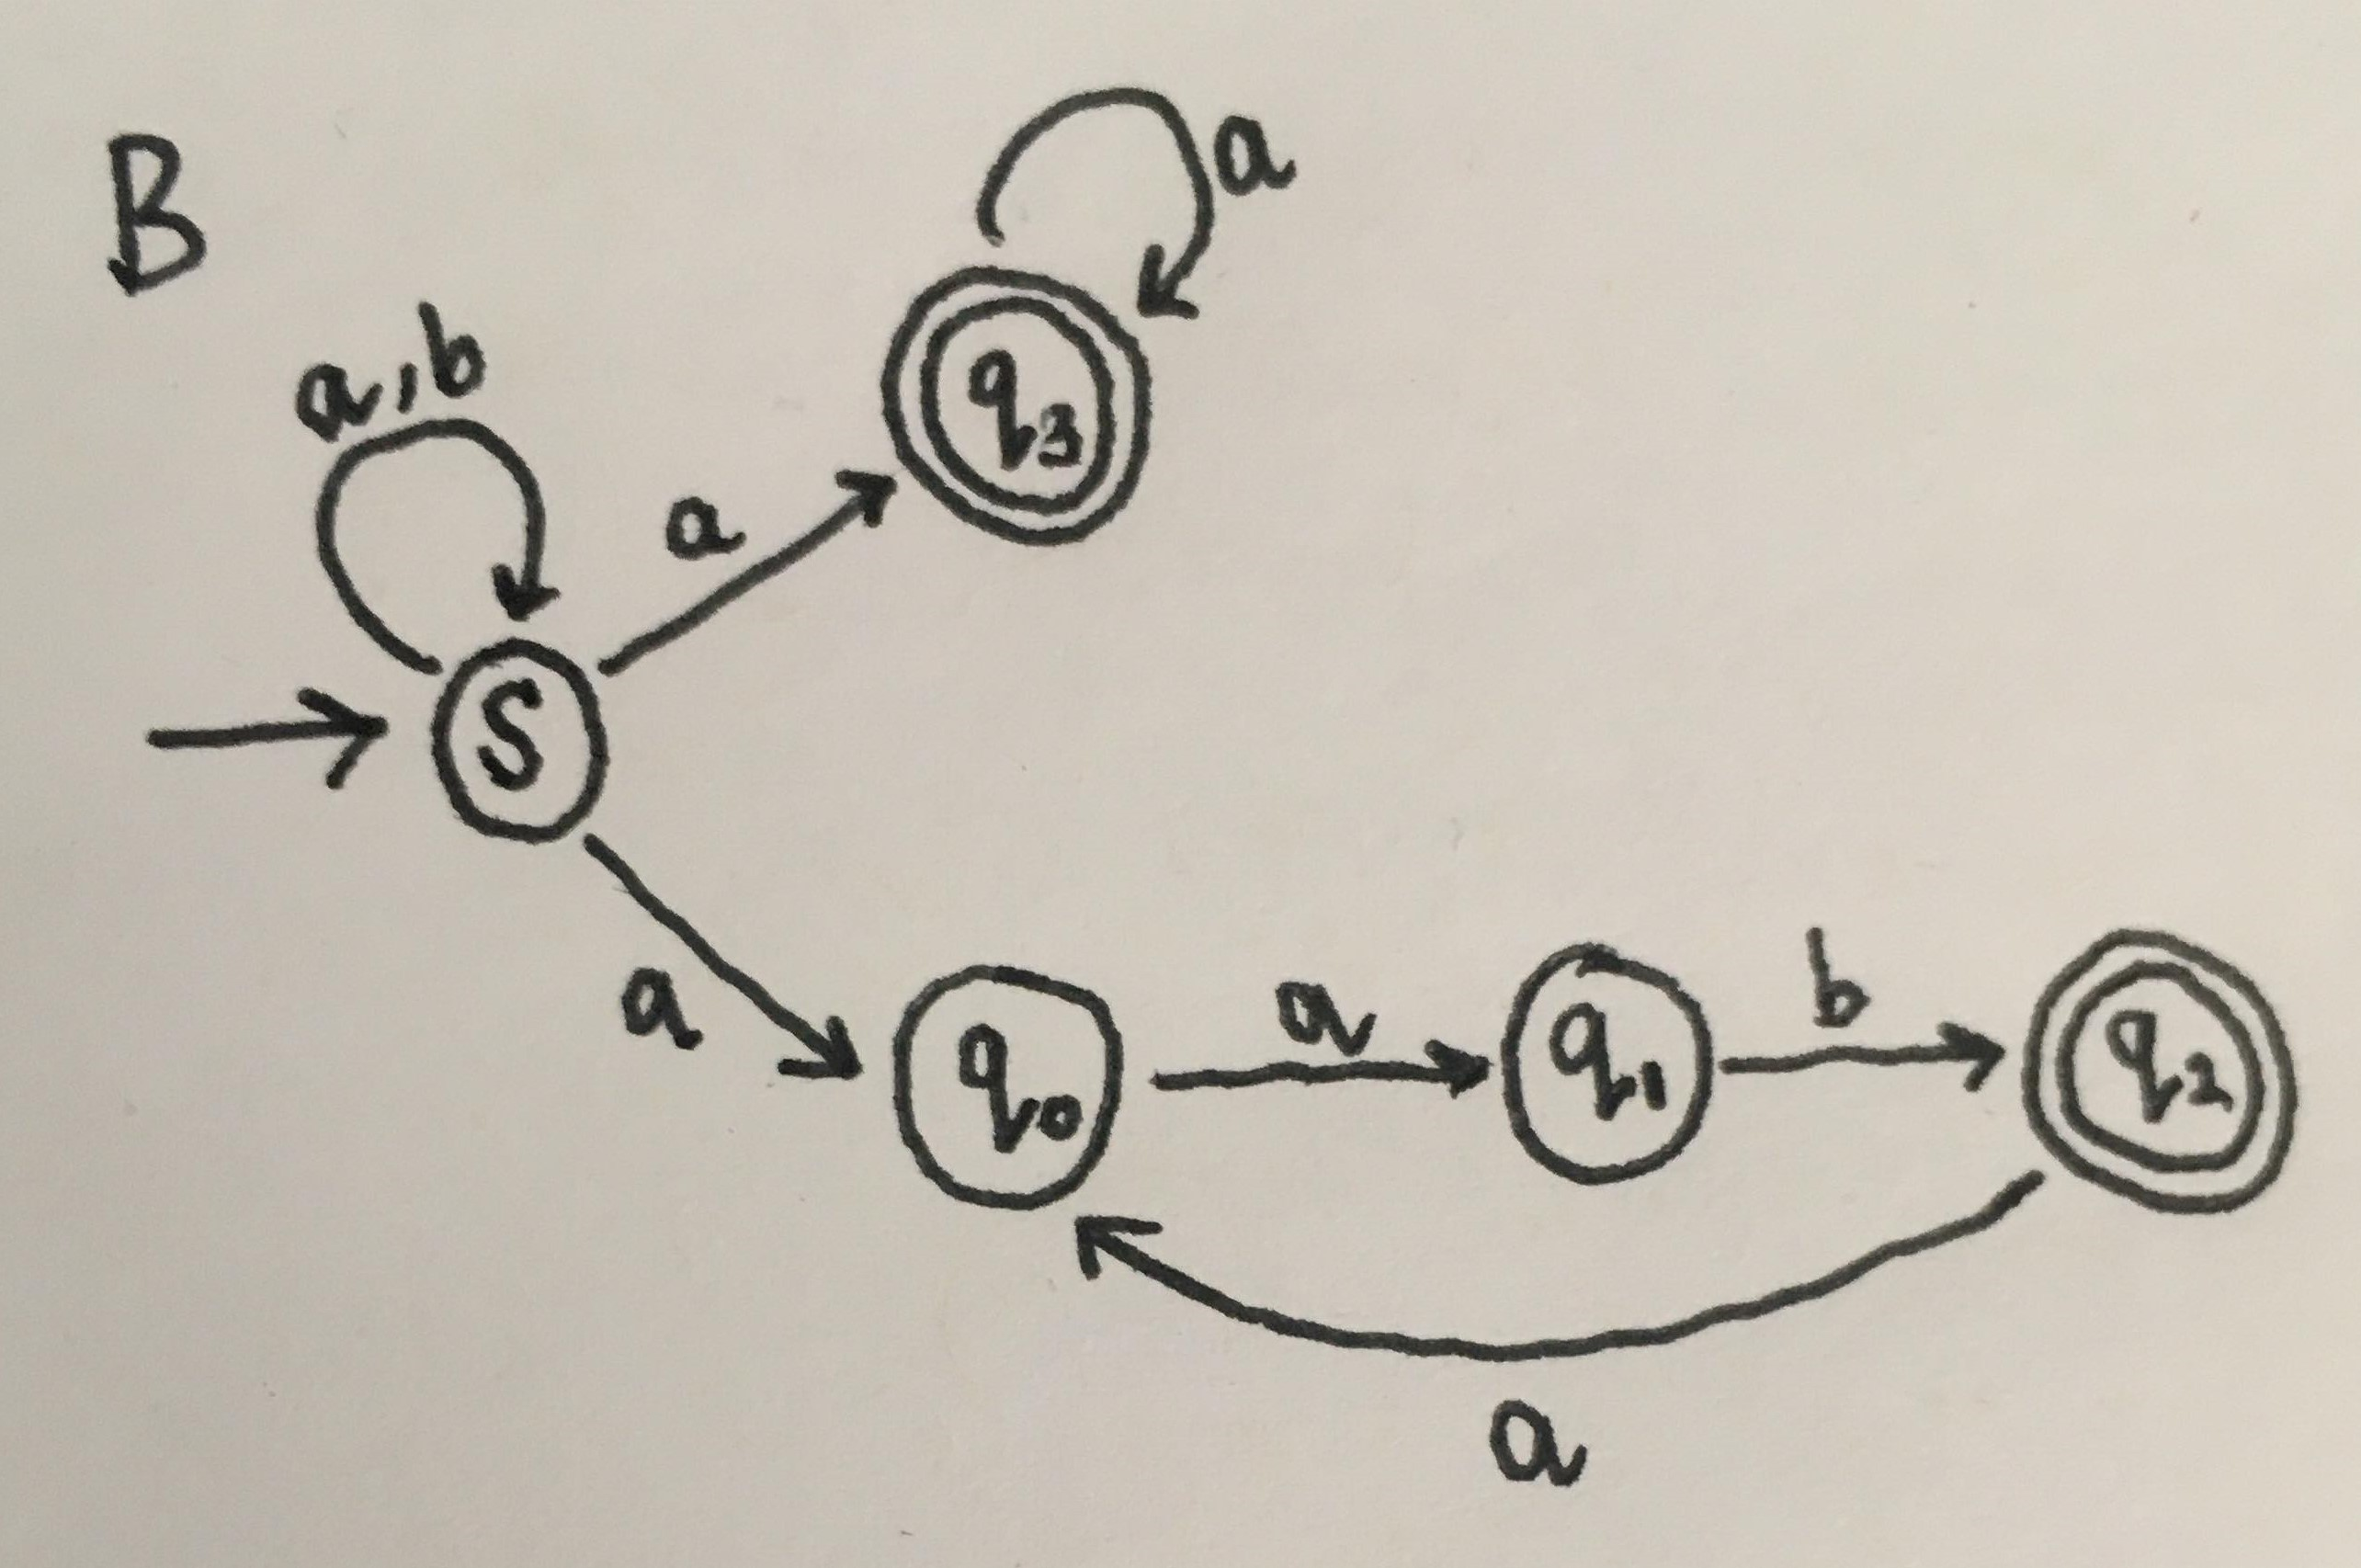
\includegraphics[width=300px]{figure1.7.jpg}
\caption{A Transition Diagram of $B$}
\label{image-Figure7}
\end{figure}
\noindent [example has been extended and changed from, 10, 2.1 Büchi Acceptance, p.7-8]
\end{exmp}


\noindent For a set $A$ to be DFA-recognisable the set must be the language for some DFA D, that is $A=L(D)$. By chapter 2 we know that all DFA-recognisable sets are also NFA-recognisable and vice versa. For clarification, a set is Büchi-recognisable if said set is the language for some Büchi automaton. 

\noindent A language is an $\omega$\textbf{-language} if $L\subseteq\Sigma^\omega$. From example, \ref{1stBüchiexmp} $L=L(B)$ is an $\omega$-language since it is a set of infinite strings.  The $\omega$\textbf{-iteration} of a set $W\subseteq \Sigma^*$ is 
$W^\omega= \{\alpha\in\Sigma^\omega \mid x_0x_1x_2...$ where $ x_i \in W$  for each $i\in\omega\}$.

For example on $\Sigma =\{a,b\}$ if $W=\{x \mid x=ba^+\}$ which is an infinite set of finite strings ($W\subseteq \Sigma^*)$. Then $baabababaaaa...\in W^\omega$ alongside any infinite string which starts with a $b$ and every $b$ is followed by at least one $a$.
\smallskip

\begin{exmp}
The $\omega$-language $L=\{\alpha\}$ over $\Sigma=\{a,b\}$ with $\alpha=abaabaaabaaaab...$ is not Büchi recognisable. 


Proof: suppose $L$ is Büchi recognisable, that is $L(B)=\{\alpha\}$ for some Büchi automaton $B$.
Then there exists some successful run $r_1=q_0q_1q_2.....$ on $\alpha$. (Note consecutive states of the run are indexed by $\omega$ but $q_i$'s are not all distinct since $Q$ is a finite set.) $r_1$ is successful so it visits some $q_f \in F$ infinitely many times. Let $0\leq k< k'$ be the first and second time the run visits $q_f$, that is $q_k=q_{k'}=q_f$. 
Then there exists another successful run $r_2=q_0...q_{k-1}(q_k.....q_{k'})^\omega$ on input $\alpha_2=\alpha(0)...\alpha(k-1)(\alpha(k)...\alpha(k'))^\omega $ with  $\alpha_2 \neq  \alpha$. This contradicts $L$ being a singleton set and hence $L$ is not Büchi recognisable. ($\alpha_2 \neq  \alpha$ since the incremental increase of $a$ between two successive $b$'s in $\alpha$ does not occur in $\alpha_2$. This is because $\alpha_2$ ends in a repeating pattern from symbol $k$ to symbol $k'$ whereas $\alpha_2$ pattern does not repeat.) 
\noindent [8, Büchi Automata, p.2]
\end{exmp}

\begin{note}
This is the first example of how the properties and characteristics of Büchi automaton are not analogous to that of an DFA or NFA. In the context of finite strings, all finite languages can be represented by regular expressions and hence are DFA/NFA recognisable, but as shown in the example above, in the context of infinite strings, not all finite languages are Büchi recognisable. 
\end{note}


\begin{definition}
A $\omega$-language ($L\subseteq \Sigma^\omega$) is $\omega$-regular if it is of the form $\bigcup_{1=0}^{n} V_i(W_i^\omega)$, where $V_0, ..., V_n, W_0, ..., W_n \subseteq \Sigma^*$ are finitely many DFA/NFA-recognisable sets, (finitely many regular languages). 


\noindent[9, Büchi automata, p.6]
\end{definition}


\begin{theorem}(Büchi's Characterization Theorem(1962))
An $\omega$-language is Büchi recognisable if and only if it is $\omega$-regular. 


\noindent[8, $\omega$-regular Languages, p.6]
\end{theorem}


\begin{proof}
($\impliedby$) Assume that an $\omega$-language is $\omega$-regular then we will show it is Büchi recognisable. We need to prove the three claims below to construct this proof:
\begin{enumerate}
\item If $W_i\subseteq \Sigma^*$ is a regular language (DFA/NFA-recognisable) then $W_i^\omega\subseteq\Sigma^\omega$ is Büchi recognisable.
\item If $V_i\subseteq \Sigma^*$ is a regular language and $K\subseteq \Sigma^\omega$ is Büchi-recognisable then $V_iK\subseteq \Sigma^\omega$ is Büchi-recognisable. 
\item If $L_1$ and $L_2$ are Büchi-recognisable subsets of $\Sigma^\omega$, then so is $L_1\cup L_2$. 
\end{enumerate}
From this it follows that every language of the form $\bigcup_{1=0}^{n} V_i(W_i^\omega)$ i.e. every  $\omega$-regular language, is Büchi-recognisable. 
Proof of claims:

Proof 1. Assume $W_i\subseteq\Sigma^*$ is DFA/NFA-recognisable. That is $L(M)=W_i$ for some DFA $M$ where $M=(Q,\Sigma, \delta, q_0, F)$. We make the added assumption that $M$ has no transitions from any other state to $q_0$, the initial state. This assumption is valid since if there were transitions to the start state, we can adapt the automaton by the addition of a new start state with an $\varepsilon$-transition to the old start state $q_0$. Although this creates an $\varepsilon$-BA this does not matter as there is an equivalent BA. 

So now we have $M$ with no transitions to $q_0$. We define the NFA $B$, by $B=(Q,\Sigma,\Delta,\{q_0\}, \{q_0\})$. Where 

$\Delta(q,a) = 
\begin{cases}
\{\delta(q,a)\} \text{ if } \delta(q,a)\notin F \\
\{\delta(q,a),q_0\} \text{ if } \delta(q,a)\in F
\end{cases}$

On input $\alpha\in\Sigma^\omega$ each time $B$ reaches a state which, in $M$ transitions to a final state in $F$, $B$ non-deterministically decides either to continue as it would in $M$ or to transition to the start state $q_0$ and continuing reading the infinite word. Now it is left to show the language of $B$ is $W_i^\omega$.


Let $\alpha\in W_i^\omega$ then $\alpha$ can be partitioned into substrings $\alpha=w_0w_1... $ where each $w_i \in W_i=L(M)$. This means each substring $w_i$ is accepted by $M$. Such a substring $w_i$ produces a run $p_{0,i}p_{1,i}...p_{n,i}$ of $M$ which obeys 
\begin{itemize}
\item $p_{0,i}=q_0$
\item $p_{j+1,i}=\delta(p_{j,i},a_{j,i})$, for $j\in \mathbb{N}$
\item $p_{n,i}\in F$ 
\end{itemize}

We know the run $r= p_{0,0}...p_{(n-1),0} p_{0,1}...p_{(n-1),1} p_{0,2}....= q_0...p_{(n-1),1} q_0...p_{(n-1),1} q_2...$ exists on $\alpha$ by definition of $B$. Moreover this is a successful run as $In(r) \cap F = In(r) \cap \{q_0\} \neq \emptyset$ so  $\alpha\in L(B)$. This means since $\alpha\in W_i^\omega$ was arbitrary, $W_i^\omega\subseteq L(B)$.


Now let $\alpha \in L(B)$, which means there is a run $r$ of $B$ on $\alpha=a_0a_1....$ which must start at $q_0$ and occur there infinitely many times ($In(r)\cap F \neq\emptyset$). 
In $\alpha$, each time $B$ arrives at $q_0$ there exists  $q_0\in \Delta (q_{t_i},a_{t_i})$ where $i\in\{0,1,...\}$. By the definition of $B$ (and by our assumption on $M$) $\delta(q_{t_i},a_{t_i})=q_f$ for $q_f\in F$. Hence we partition $\alpha$ as $\alpha(0)...\alpha(t_0)$, $\alpha(t_{0}+1)...\alpha(t_1)$, $\alpha(t_1+1)......$. Since $\alpha(0)=q_0$ and $\alpha(t_i)=a_{t_i}$ each of these partitioned strings are accepted in $M$. Hence $L(B)\subseteq W_i^\omega$.

So, $L(B)=W_i^\omega$ as required.
[10, 2.1, p.8.9]

2. Assume $V_i\subseteq \Sigma^*$ is a regular language and $K\subseteq \Sigma^\omega$ is Büchi-recognisable.
Let $M=(Q_M, \Sigma, \delta, q_0, F_M)$ be a DFA with $L(M)=V_i$ and let $B=(Q_B,\Sigma,\Delta_B, S_B, F_B)$ be a BA with $L(B)=K$. We assume $Q_M\cap Q_B=\emptyset$ and define the BA $C=(Q,\Sigma, \Delta, \{q_0\},F_B)$ where $Q=Q_M\cup Q_B$, the start state of $C$ is the start state of $M$, the final states of $C$ are those of $B$. Lastly, the transition function has all transitions of $B$ and $M$ but when $C$ is at a state which can transition to a final state of $M$, it has the additional option to transition to a start state of $B$. The transition function is given by,


$\Delta(q,a) =
\begin{cases}
\{\delta(q,a)\} \text{ if } q\in Q_M\text{ and } \delta(q,a)\notin F_M\\
\{\delta(q,a)\}\cup S_B \text{ if } q\in Q_M \text{ and } \delta(q,a)\in F_M \\
\Delta_B(q,a) \text{ if } q\in Q_B
\end{cases}$

An arbitrary successful run of $C$ on $\alpha\in\Sigma^\omega$ has the form: starts in $M$ since $C$ and $M$ share the same start state, undergoes a successful run $r_{v_i }\in V_i$ of $M$ in order to transition to $B$, then 
as $C$ and $B$ share the same final states it must follow a successful run $r_k\in K$ of $B$ in order for $In(r) \cap F_B\neq\emptyset$ . Hence every successful run is of the form $V_iK$. 

Conversely, let $r$ be an arbitrary run of the form $V_iK$ which means we can partition it by $r=r_{v_i}r_{k}$. This run $r$ is legal on $C$ as it starts at $M$, and therefore $C$, start state $q_0$ and all states visited are in $Q$. In $C$ on $r$ since $r_{v_i}\in V_i$ is an accepting run of $M$ before $r_{v_i}$ transitions to the final state of $M$ it can transition to a start state of $B$ where $r_k$ is then read and since $r_k\in K$ is accepted by $B$, $r_k$ is accepted by $C$. Hence $r$ is accepted by $C$. Hence, $L(C)=V_iK$  i.e. $V_iK\subseteq \Sigma^\omega$ is Büchi-recognisable. 
[3]

3. Assume $L_1$ and $L_2$ are Büchi-recognisable, that is there are two BA, $B_1=(Q_{B_1},\Sigma,\Delta_{B_1},S_{B_1},F_{B_1})$ and $B_2=(Q_{B_2},\Sigma,\Delta_{B_2}, S_{B_2}, F_{B_2})$ with $L(B_1)=L_1$ and $L(B_2)=L_2$ (w.l.o.g assume $Q_{B_1} \cap Q_{B_2}=\emptyset$). We create a new BA $B$ whose language will be shown to be $L(B)=L_1\cup L_2$. Let $B=(Q_B, \Sigma, \Delta, s,  F_B)$ where $Q_B=Q_{B_1}\cup Q_{B_2}\cup s$ and $F_B=F_{B_1}\cup F_{B_2}$. Moreover for  $a\in\Sigma$, $q\in Q_B$ we have

 
$\Delta(q,a) = 
\begin{cases}
 \Delta_{B_1}(q,a) \text{ if } q\in Q_{B_1}\\
 \Delta_{B_2}(q,a) \text{ if } q\in Q_{B_2} \\
 \emptyset \text{ if } q=s \\
\end{cases}$
$\Delta(q,\varepsilon) = 
\begin{cases}
\{ S_{B_1}, S_{B_2} \}\text{ if } q= s\\
\emptyset \text{ if } q\neq s \\
\end{cases}
$

Which allows $B$ on any infinite word $\alpha$ to $\varepsilon$-transition and be read along $B_1$ where it will only be accepted if $B_1$ accepts $\alpha$. Or $\varepsilon$-transition and be read along $B_2$ where it will only be accepted if $B_2$ accepts $\alpha$.  Hence its language is the union of $B_1$ and $B_2$ languages. More formally, $L(B) \subseteq L_1 \cup L_2$ since for $\alpha\in L(B)$ with an accepting run $r=sq_0q_1q_2...$ in $B$, if $q_0 \in S_{B_1}$ then $r$ is an accepting run on $B_1$, else $q_0 \in S_{B_2}$ and $r$ is an accepting run on $B_2$. Moreover, $L(B) \supseteq L_1 \cup L_2$ since for $i\in\{1,2\}$ and $\alpha\in L(B_i)$, then there is an accepting run $r$ on $B_1$ hence the run $r$ is accepting for $\alpha$ in $B$. 

This proof relies on the fact that $\varepsilon$-BA are equivalent to BA. An equivalent proof can be used instead which is similar to the method of proof 1. Whereby, instead of $\varepsilon$-transitions, transitions from both $B_1$ and $B_2$ start states are grouped by changing the start point of these transitions, from their individual start state to $B$ new start state and leaving the symbol and end point of the transition unchanged. 

[8, 3 $\omega$-languages, page 4]

($\implies$) Assume that an $\omega$-language is Büchi recognisable then we will show that it is $\omega$-regular.

Let $L\in\Sigma^\omega$ be the language of a BA $B$ where $B=(Q,\Sigma, \Delta,S, F)$. It accepts some infinite word $\alpha=a_1a_2a_3...$ (where $a_i\in\Sigma$). Let  $sq_1q_2.....$ be a successful run of $B$ on $\alpha$, that is $q_{i+1}\in\Delta(q_i,a_{i+1})$ for $i\in\{1,2,...\}$ and $q_1\in\Delta(s,a_1)$. Since this run is successful there is $f\in F$ such that $q_n=f$ for infinitely many $n$. So we partition $\alpha$ corresponding to a string which takes you to state $f$ and then strings which start at $f$ and finish

at $f$, (we know such a partition exists by the fact the run is successful and the acceptance conditions of BA). 

Let us rewrite the infinite word $\alpha$ as strings given by $\alpha=vw_1w_2w_3...$ which correspond to this partition, the initial string $v$ takes you from the start state to the first occurrence of $f$.  Clearly string $v$ is accepted by the NFA $N_{s,f} =(Q,\Sigma, \Delta, \{s\},\{f\})$. Furthermore each string $w_i$ is accepted by the NFA $N_{f,f}=(Q,\Sigma, \Delta, \{f\},\{f\})$. Let the corresponding languages for these NFA be denoted $W_{s,f}$ and $W_{f,f}$ respectively. That is for $a_i\in\Sigma$, 
\begin{align}
    W_{p,q} &:= \{w=a_1a_2...a_m \mid w \text{ is an accepting string of } N_{p,q}\}\notag \\
    &:= \{ w=a_1a_2...a_m \mid w \text{ there is a run from start state p to final state q}\} \notag
\end{align}

By above if $\alpha$ is accepted by $B$ then for some $s\in S$, $f\in F$ we have $\alpha\in W_{s,f}(W_{f,f})^\omega$. The language of $B$ is all the accepted infinite words and the maximum possible size of $L(B)$ is the union of such strings over $S$ and $F$. So we have $L(B) \subseteq  \bigcup_{s\in S, f\in F} W_{s,f}(W_{f,f})^\omega$.

If $\alpha\in\bigcup_{s\in S, f\in F} W_{s,f}(W_{f,f})^\omega$ then $\alpha=vw_1w_2w_3...$ where $v\in W_{s,f}$ and $w_i\in W_{f,f,}$ for any arbitrary $s\in S $ and $f\in F$. This means there is $N_{s,f}$ which accepts $v$ ($v$ produces a run of $s$ to $f$) and $N_{f,f}$ which accepts $w_i$ (each $w_i$ produces a run from $f$ to $f$). Since the consecutive $w_i$ in $\alpha$ satisfy the Büchi acceptance condition, $\alpha$ is a successful run of $B$ and $\alpha\in L(B)$ meaning $L(B) \supseteq  \bigcup_{s\in S, f\in F} W_{s,f}(W_{f,f}^\omega)$.

Thus we have $L=L(B)=\bigcup_{s\in S, f\in F} W_{s,f}(W_{f,f}^\omega)=\bigcup_{i=1}^{n} V_iW_i^\omega$ for $V_i$, $W_i$ regular languages.
[3][10, section 2.1, p.9]
\end{proof}

\begin{note}
A relevant application of Büchi automata is in modelling the behaviour of cancer stages. Since cancer is uncontrollable cell division this can be thought of in computing terms as an infinity loop. The stages of a cell cycle can be broken down into cell growth, replication, doubling and division. Each of these stages can be represented by a finite automaton. Then a Büchi automaton combining these four automata facilitates all the stages of a cancer cell and the fact that cell division occurs infinitely many times and hence can represent cancer progression. [14]
\end{note}


\section{Muller Automaton}
Like a BA, a Muller automaton refers to a nondeterministic automaton with inputs over infinite words, (again deterministic Muller automaton exist but will be referred to explicitly). A Muller Automaton $A$ is defined by a NFA $A=(Q,\Sigma, \Delta,S,\mathcal{F})$ with $\mathcal{F}\subseteq P(Q)$ defining a different acceptance condition:

\begin{definition}
$A$ \textbf{accepts} $\alpha\in\Sigma^\omega$ iff there is a run $r$ of $A$ on $\alpha$ such that $In(r)\in \mathcal{F}$. This means the set of states which are visited infinitely often is a member of the set of final states $\mathcal{F}\subseteq P(Q)$.
\noindent [10,2.2 Muller Acceptance, p.10][11,Formal definition]
\end{definition}

\begin{note}
$\mathcal{F}$ is also called an acceptance table with $\mathcal{F}=\{F_1,F_2,...,F_t\}$ where $F_i \subseteq Q \text{ for } i\in\{1,2,...,t\}$. $\mathcal{F}$ is a set of accepting subsets and a run $r$ of the automaton is successful if $In(r)=F_i$ for some $i\in\{1,2,...,t\}$. The acceptance condition of a Muller automaton gives more flexibility on the requirements for accepted runs as it allows for more specific runs to be accepted. The states which are visited infinitely often must be exactly the states in the set $F_i$ for some $i$. No other states can be visited infinitely often, meaning all states $Q/F_i$ must be visited finitely often. This is a more stringent condition than the Büchi acceptance condition which allows non final states to be visited infinitely often, so long as one or more states in the accepting set are visited infinitely often. 
[9, 3 Stronger acceptance conditions, p.14]
\end{note}

\begin{exmp}
In this example, I highlight different Muller automata can have the same transition diagram. This is due to each automaton $A_i \text{ for } i\in\{1,2,...,6\}$ having a different Muller acceptance (acceptance table) and the fact that acceptance is not shown on a transition diagram, instead table $\mathcal{F}_i$ is given. For each 
$A_i=(Q,\Sigma, \Delta, S, \mathcal{F}_i)$ we have $Q=\{s,q\}, \Sigma=\{a,b\},$  $\Delta$ is given in figure 4.2, $S=\{s\}$ and $\mathcal{F}_i\subseteq P(Q)=\{\{s\},\{q\},\{s,q\}\}$. So the total possible Muller acceptance conditions $\mathcal{F}_i$ are, 

\noindent - $\mathcal{F}_1=\{\{s\}\}$. On a successful run $r$ of $A_1$ we must have $In(r)=\{s\}$ so there must be infinitely many $a$'s and finitely many $b$'s. That is, $L(A_1)=(a+b)^*a^\omega$.


\noindent - $\mathcal{F}_2=\{\{q\}\}$. Similarly to $A_1$, $A_2$ accepts infinite words with infinitely many $b$'s and finitely many $a$'s giving, $L(A_2)=(a+b)^*b^\omega$

\noindent - $\mathcal{F}_3=\{\{s\},\{q\}\}$. On a successful run $r$ of $A_3$ we must have either $In(r)=\{s\}$ or  $In(r)=\{q\}$ so strings must have infinitely many $a$'s and finitely many $b$'s or infinite many $b$'s and finitely many $a$'s. Note $A_3$ does not accept strings with infinitely many $a$'s and $b$'s. $L(A_3)= (a+b)^*a^\omega + (a+b)^*b^\omega$.

\noindent - $\mathcal{F}_4=\{\{s,q\}\}$. Again this means $In(r)=\{s,q\}$ for some successful run which means an accepting word must contain both infinitely many $a$'s and infinitely many $b$'s, $L(A_4)=(a+b)^*b(a+b)^*a)^\omega$ .

\noindent - $\mathcal{F}_5=\{\{s\},\{s,q\}\}$. Combination of the fact an accepting run has either $In(r)=\{s,q\}$ or $In(r)=\{s\}$ means $r$ can have either infinitely many $a$'s and finitely many $b$'s, or infinitely many $a$'s and infinitely many $b$'s. Hence $L(A_5)=\{\alpha \mid \alpha \text{ has infinitely many } a\text{'s }\}=(b^*a)^\omega$

\noindent - $\mathcal{F}_6=\{\{q\},\{s,q\}\}$. Similarly, $L(A_6)=\{\alpha \mid \alpha \text{ has infinitely many } b\text{'s }\}=(a^*b)^\omega$

\noindent - $\mathcal{F}_7=\{\{s\},\{q\},\{s,q\}\}$. $L(A_7)= \{\alpha\mid\alpha\in\Sigma^\omega\}$.

\noindent - $\mathcal{F}_8=\emptyset$. No infinite words are accepted hence $L(A_8)= \emptyset$.



\begin{figure}[ht]
\centering
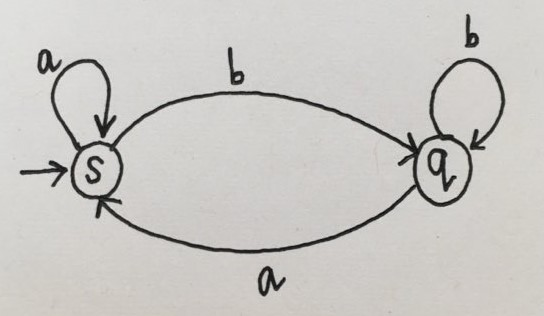
\includegraphics[width=300px]{figure1.8.jpg}
\caption{Muller automaton $A_i$}
\label{image-Figure8}
\end{figure}
\end{exmp}
[Transition diagram and two $\mathcal{F}$ tables were expanded and added too from 12, 6, p.1]

\begin{theorem}
For every Büchi automaton $B$ there is a Muller automaton $A$ such that $L(B)=L(A)$. [13, slide 43]
\end{theorem}
\begin{proof}
Let $B=(Q,\Sigma,\Delta,S,F)$ and we define $A$ to have the same automaton graph as $B$ and the acceptance condition $\mathcal{F}=\{X\in P(Q) \mid X\cap F \neq\emptyset\}$ (where $P(Q)$ is the power set of the states of $B$ (and $A$)). That is $A=(Q,\Sigma,\Delta, S, \mathcal{F})$. 

Let $\alpha\in \Sigma^\omega$ be any infinite word accepted by $B$. Then there exists a successful run $r$ of $B$ on $\alpha$ with $In(r) \cap F\neq\emptyset$ and since $In(r)\in P(Q)$ (because all elements of $In(r)$ are in $Q$) the set $In(r)\in\mathcal{F}$, by definition of $\mathcal{F}$. Hence $r$ is a successful run of $A$ and $\alpha$ is accepted by $A$. 

Let $\alpha\in\Sigma^\omega$ be any infinite word not accepted by $B$.  Then there does not exist a successful run of $B$ on $\alpha$, which means for all runs $r$ on $\alpha$ we have $In(r)\cap F = \emptyset$, thus $In(r) \notin \mathcal{F} $ and hence $\alpha$ is not accepted by $A$. 
Hence $L(B)\subseteq L(A)$. The converse argument is analogous. In summary, for $\alpha\in\Sigma^\omega$ and some run $r$ on $\alpha$, 
$\alpha\in L(A)\iff In(r)\in \mathcal{F}\iff In(r) \cap F \neq\emptyset \iff \alpha\in L(B)$. 
Hence $L(A)=L(B)$.
\end{proof}
[13, slide 44]

\begin{note}
The theorem above holds for deterministic automata too; for every deterministic BA there exits a deterministic Muller automata. This is because the theorem and proof do not introduce or remove nondeterministic properties. [9, simulations, p.15]
\end{note}


\begin{theorem}
\label{ThmMuller->Büchi}
For every Muller automaton $A$ there is a Büchi automaton $B$ such that $L(A)=L(B)$. [12, theorem 2, p.1]
\end{theorem}

\begin{proof}
Let $A=(Q,\Sigma,\Delta,S,\mathcal{F})$ be a Muller automaton with $\mathcal{F}=\{F_1,F_2,...,F_t\}$. We construct a BA $B_i$ for each $i\in\{0,1,...,t\}$ which accepts $\alpha\in\Sigma^\omega$ iff there is an accepting run $r$ on $A$ of $\alpha$ with $In(r)=F_i$. Then we have $L(A)=\bigcup_{i\in\{1,2,...,t\}} L(B_i)=L(B)$ and by claim 3 in theorem 4.1 we know $L(B)$ is Büchi recognisable iff all $L(B_i)$ are Büchi recognisable. 

The construction of $B_i=(Q_i,\Sigma, \Delta_i, S_i, G_i)$ is given below for $F_i=\{f_{i_1},f_{i_2},....,f_{i_m}\}$. 

$Q_i=\{(q, finite) \mid q\in Q \} \cup \{(f, infinite, j) \mid f\in F_i \text{ and } j\in\{0,1,...,m-1\}\}$

$S_i=\{(s, finite)\mid s\in S\}$

$G_i=\{(f_{i_m}, infinite, m-1)\} $

$\Delta_i((q,finite),a)=
\begin{cases}
(q',finite)  \text{ if }\Delta(q,a)=q'\\
(q',infinite,0)  \text{ if } \Delta(q,a)=q' \text{ and } q'\in F_i
\end{cases} $

$\Delta_i((q,infinite,k),a) =
\begin{cases}
(q',infinite,k) \text{ if }\Delta(q,a)=q'\text{ and } q'\in F_i \text{ and } q\neq f_{i_{k+1}}\\
(q',infinite,(k+1)\mod m )  \text{ if }\Delta(q,a)=q', q'\in F_i \text{ and } q=f_{i_{k+1}}
\end{cases}$ 

States of $B_i$ are categorised into two groups: states which are visited finitely often, shown by ordered pairs and states which are visited infinitely often, denoted by a 3-tuple. Since any state in $A$ could be finitely visited all states from $A$ are given as an ordered pair. For the 3-tuples, we only want states in $F_i$ to be infinitely visited and for each state of $F_i$ we create $F_i$ many variations of this state in $B_i$. This is denoted by the third entry which acts as an alternator/ counter for states being visited infinitely often in $B_i$. 

The start state $S_i$ are the ordered pairs of the start states of $A_i$. If a start state $s$ of $A_i$ is visited infinitely often this is broken down in $B_i$ by the state $(s,finite)$ as a start state and the state $(s, infinte, j)\mid j\in\{0,1,...|F_i|\}$ accounts for the rest. 

The transition functions $\Delta_i$ encapsulates that at some point $A_i$ non deterministically decides no more states from $S/F_i$ will be visited, after this point $A_i$ transition's are within $F_i$ only whilst visiting all the states infinitely often. $\Delta_i$ mirrors $\Delta$ transitions for all states visited finitely often in $A$. Then when $\Delta$ transitions to a state in $F_i$, $\Delta_i$ then transitions between infinite states only. The third entry of the tuple, $k$, acts as a counter which keeps $B$ moving within all the infinite states (this is due to the condition $q=f_{i_k+1}$ or $q\neq f_{i_k+1}$). In order for a run $\alpha$ to be accepted in $A$ it must visit all $f_{i_j}$ for $ j\in\{0,1,...m\}$ infinitely often, the counter $k$ and inequality conditions mean if $(f_{i_m}, infinite, m-1)$ is being visited infinitely often (with counter $k$ at its largest value of $m-1$), then all of the infinite states of $A$ are, hence the run is accepted in $A$. So we set $G_i$ to be said state and hence the run is accepted in $B_i$. 
It is stated without further proof that from the construction of $B_i$ if $\alpha\in\Sigma^\omega$ is an accepted string in $B_i$ then $\alpha$ has a run on $A$ with $In(r)=F_i$. 

Hence a string is accepted by  $L(B_i)$ iff there is a run on $A$ of the string with $In(r)=F_i$ as required. 
\end{proof}
[Proof has been followed closely from 9, simulations, p.15-16] [13, slides 48-51]

The next theorem is given without proof.
\begin{theorem}(McNaughton)
For every Büchi Automaton $B$ there is an equivalent deterministic Muller Automaton $A$. Every $\omega$-regular language is recognised by a deterministic Muller Automaton. 

[9, 3, p.16]
\end{theorem}

\medskip
By theorem 4.2 and 4.3 we have shown that Muller and Büchi automata are equivalent. We also have from McNaughten's theorem an inclination of deterministic Muller automata power.  It turns out that Muller and non deterministic Muller automata are equivalent [3]. Hence combining these two statements gives an equivalence of (non deterministic) Muller, (non deterministic) Büchi and deterministic Muller automata. 
This is significant since deterministic and non deterministic Büchi automata are not equivalent [3]. Hence this shows that Muller automata (deterministic and non deterministic) are more powerful since they recognise all $\omega$-languages whereas deterministic Büchi automata can be viewed as weaker as they do not. 
[9, simulations, p.14]














\chapter{References}
[1] Hopcroft, J., Motwani, R., \& Ullman, J. (2007). Introduction to automata theory, languages, and computation  (Third edition.). Pearson/Addison Wesley.


\noindent[2] Automata Theory Introduction. \url{https://www.tutorialspoint.com/automata_theory/automata_theory_introduction.htm}

\noindent[3] Paul Shafer Lecture Notes.

\noindent[4] Kelley, D. (1995). Automata and formal languages: an introduction. Prentice Hall.

\noindent[5] Carroll, J., \& Long, D. (1989). Theory of finite automata: with an introduction to formal languages. Prentice-Hall.

\noindent[6] C.Kozen, D. (1997). Automata and Computability. Springer.

\noindent[7]  Büchi wikipedia page. \url{https://en.wikipedia.org/wiki/B%C3%BCchi_automaton}

\noindent[8] Automata, Games, and Verification: Lecture 2.
Bernd Finkbeiner.
\url{https://www.react.uni-saarland.de/teaching/automata-games-verification-12/downloads/notes2.pdf}

\noindent[9] Finite-state Automata on Infinite Inputs.
Madhavan Mukund.
\url{https://www.imsc.res.in/~madhavan/papers/pdf/tcs-96-2.pdf}

\noindent[10] Finite $\omega$-Automata and Büchi Automata.
Abdulla Eid.
\url{https://faculty.math.illinois.edu/~eid1/ba.pdf}

\noindent[11] Muller wikipedia page.
\url{https://en.wikipedia.org/wiki/Muller_automaton}

\noindent[12] Automata, Games, and Verification: Lecture 5.
Bernd Finkbeiner.
\url{ https://www.react.uni-saarland.de/teaching/automata-games-verification-12/downloads/notes5.pdf}

\noindent[13] Automata on Infinite Words.
Paritosh K. Pandya.
\url{http://www.tcs.tifr.res.in/~pandya/grad/aut06/lect4.pdf}

\noindent[14] Singh, N., \& Kumar, A. (2018). Modelling finite and infinite behaviour of cancer stages using Buchi and finite automata. Current Science (Bangalore), 115(4), 677–681. https://doi.org/10.18520/cs/v115/i4/677-681

\end{document}




